% https://www.overleaf.com/read/jydxqkkkskzp
% https://github.com/MCG-NKU/NSFC-LaTex
% by Ming-Ming Cheng https://mmcheng.net

\documentclass[12pt]{article}
\usepackage[UTF8]{ctex}
\usepackage{nsfc}
\usepackage{url}
\def\UrlBreaks{\do\A\do\B\do\C\do\D\do\E\do\F\do\G\do\H\do\I\do\J
\do\K\do\L\do\M\do\N\do\O\do\P\do\Q\do\R\do\S\do\T\do\U\do\V
\do\W\do\X\do\Y\do\Z\do\[\do\\\do\]\do\^\do\_\do\`\do\a\do\b
\do\c\do\d\do\e\do\f\do\g\do\h\do\i\do\j\do\k\do\l\do\m\do\n
\do\o\do\p\do\q\do\r\do\s\do\t\do\u\do\v\do\w\do\x\do\y\do\z
\do\.\do\@\do\\\do\/\do\!\do\_\do\|\do\;\do\>\do\]\do\)\do\,
\do\?\do\'\do+\do\=\do\#} 


\newcommand{\note}[1]{\textcolor[rgb]{0.6,0,0}{note: #1}}
\newcommand{\todo}[1]{{\textcolor{red}{\bf [#1]}}}
\newcommand{\myPara}[1]{\paragraph{#1:}}

\graphicspath{{figures/}}


\begin{document}



%%%%%%%%% TITLE

\title{报告正文}
% title: 危化品智能装配中的高精度6D姿态估计方法研究
\maketitle
\thispagestyle{empty}

\ContentDes{(一)立项依据与研究内容(建议8000字以下):}


\NsfcSection{1}{项目的立项依据}{
(研究意义、国内外研究现状及发展动态分析,需结合科学研究发展趋势来论述科学意义;或结合国民经济和社会发展中迫切需要解决的关键科技问题来论述其应用前景。附主要参考文献目录);}

\subsection{研究意义}

爆炸品、有毒化工、放射性物质、生物化学制剂等危化品的装配工艺,对于制备环境要求很苛刻。工厂装配过程中,为了确保装配安全性,对产线工人的年龄、工作时间和操作流程等都有严格的要求。以工程炸药制备公司为例,为了保障安全生产,工人正常上工前需培训6个月,每天工作时间不能超过6小时,每项工艺流程需双人确认。这些安全措施极大限制了工厂的产能,亟需通过智能制造技术替代人工,提升产能。

% 此处表述6D姿态估计是智能装配中的关键技术,为了提升精度,需要用多传感器融合
待装配物件的六自由度(6D)姿态估计是智能装配的关键技术,其核心问题是高精度的姿态估计。与普通的工业自动化设备不同,危化品的装配操作流程裕度很小,无法通过降低机械操控设备的控制精度和重访精度实现无人操作。智能装配工艺通过装置在产线上的传感器,估计炸药、放射性元素、腐蚀性药品等空腔的姿态,在操控链路形成负反馈,精准完成原料装填和定位螺丝的紧固。

% 传统的6D姿态估计采用RGB或RGBD的方式计算姿态,准确度以目标物体点云的10%作为度量,无法满足精准装配的需要,亟需改进;当前的学术研究中,6D姿态估计算法估计的准确度以目标物体点云尺度的10\%作为度量,其精度只适用于普通物件如快递包裹、日常物品等的粗抓取,无法满足危化品装配的精细操控要求。
面向危化品智能装配的6D姿态估计需要解决三个核心问题,其一为弱纹理表面的算法适应性问题,其二为有遮挡情况下的鲁棒估计问题,其三为姿态估计的高精度修正问题。本项目融合可见光、深度图和光谱相机的影像特征,通过分析多模态传感器数据的特征表达,提取和对齐不同模态的特征,并通过交叉验证抑制单一模态中的噪声,融合有效的互补信息,提升6D姿态估计的适应性、鲁棒性和精度,解决危化品智能装配中的高精度姿态估计难题。

\subsection{国内外相关工作}

大多数姿态估计方法遵循两阶段的范式,首先检测图像中的目标物体,之后在缩放后的目标物体区域上进行姿态估计。尽管现有方法在大多数简单的场景下表现良好,但由于所使用的检测器对弱纹理或被遮挡工件的检测效果并不理想,算法在智能装配应用中的性能急剧下降。

对于第一阶段的目标检测任务,常用的检测方法有两段式和单段式两类\cite{ATSS, fcosv1, fcosv2, PAA, faster-rcnn, maskrcnn}。两段式检测方法首先采用区域建议网络~\cite{faster-rcnn, maskrcnn}生成边界框候选体,然后由分类和细化网络处理,去除假阳性,并调整边界框的位置和大小。这种策略准确度较高,但成本高,效率低。单段式检测器通过在编码器的最终特征图中的每个空间位置用一组预定义的锚框代替区域建议网络来解决这个问题~\cite{retinanet,fcosv1,yolov1}。这种方法会导致锚点中存在大量负样本,虽然这一问题可以通过focal loss~\cite{retinanet,fpn}在一定程度上解决,但程度有限,早期的单段式检测器并没有达到两段式检测器的精度。Zhang~\cite{ATSS}通过一个简单而有效的正样本策略解决了这一问题。最近的大多数检测方法都遵循类似的策略~\cite{fcosv2, PAA, autoassign, OTA, TTF, yolov3},相关改进算法的准确性比两段式方法更好,同时效率更高。但即便如此,这些方法都假设场景中物体的纹理相对丰富,且具有较少的遮挡,与智能装配的6D物体姿态估计场景中的特性仍有较大差异。

% 弱纹理物体位姿估计解决方案:在数据输入源头上解决,即增加depth图像和高光谱图像,实现多源融合。
危化品工件的表面大多没有纹理,这种工况下的目标检测是姿态估计中的一个难点。仅通过RGB图像估计的位姿精度不高,鲁棒性较差。一方面,深度学习网络很难从单幅RGB图像中提取有效的颜色和几何特征,另一方面,三维物体到二维像平面的投影过程丢失了三维结构的几何约束,单幅图像无法逆推结构信息。
基于RGB-D的6D位姿估计方法可以利用点云的三维几何特征来预测目标姿态,其估计精度比单幅RGB图像更高。这类算法的难点在于RGB图和深度图两种异构数据的融和。目前解决的思路有三类。
第一类为像素级融合方法,先利用2D检测或分割网络提取RGB图像特征,将图像特征传递给深度图生成的点云,然后将增强后的点云反馈给点云3D目标检测器。2D检测的结果可辅助三维点云形成3D视锥\cite{Qi2018},减小候选区域的范围。所形成的的视锥也可以进一步划分为网格单元\cite{Wang2019}进行3D检测。或者2D分割的结果也可用于增强3D点云\cite{Vora2020},将增强后的点云输入3D目标检测器提升检测效果。这类方法以顺序的方式进行融合,效率相对较低。
第二类为特征级融合方法,在基于点云的3D目标检测器的中间阶段融合图像和点云特征。例如,在基于网格的检测网络骨干的中间层中使用连续卷积\cite{Liang2018, Liang2019}、混合体素特征编码\cite{Sindagi2019}或Transformer\cite{Zhang2022}网络等融合算子进行多模态融合。
第三类为决策级融合,将RGB图像和Depth图像生成的点云数据通过两个独立网络分别生成2D和3D检测框\cite{Asvadi2018}并融合输出。这种方法可以更好地借鉴每个独立任务的SOTA算法,避免中间特征层上的信息交互,执行效率高,但无法利用不同模式的互补语义信息\cite{Pang2020}提升检测精度。

%本项目在特征级融合的基础上,引入UV数据保持深度图点特征三维空间位置的一致性,从而在异构输入源之间解决视角对齐的问题。
与普通工业零件不同,危化品工件中通常有危险度较高的化学部件,如易爆、有毒或有辐射的填充物。对于这类区域的精细检测和分割,一方面可以避免误操作减少事故,另一方面可为检测网络提供更精准的边界区域特征。不同的化学元素在特定的光谱谱段有脉冲响应特性,可通过光谱相机清晰地定位物质边界,能显著提升姿态估计第一阶段的检测和分割精度。光谱图像的检测和分割算法思路与可见光图像相似,最主要的问题在于样本数据较少,且分布不均匀,业界没有大规模数据集可用于网络训练。目前解决这一问题的主要方法是小样本学习\cite{lys2022targetDetection, shi2020HyperspectralTargetDetection}或加强注意力机制\cite{shi2020hyperspectralROI}。

% 此处描述 RGB, Depth, 和光谱数据融合的国内外现状
对于同一场景下的可见光、深度图和光谱图像的融合处理,目前没有可直接借鉴的方法,但多传感器融合的方法在遥感影像处理和自动驾驶领域\cite{Feng_2021}中都有相关研究。一种朴素的融合方法是决策级融合,对不同的输入数据分别提取特征图\cite{pang2020clocs},构建基于统计的特征加权组合模块,对不同输入分支提取的特征赋予不同的权重,在输出层进行决策级融合\cite{li2022sal}。这种方法既可以区分不同输入源特征在分类器中的重要性,又可以避免特征提取网络学习本身对分类结果的干扰。但它没有考虑多源数据特征间的差异性与互补性。另一种思路是特征级融合,先前的研究有两种模式,其中一种模式以Xie等人提出的Pi-rcnn\cite{xie2020pircnn}和Vora等人提出的Pointpainting\cite{vora2020pointpainting}为代表,将三维点云中的每一个点投影到二维像平面,然后通过双线性插值获得对应二维图像特征。这种方式虽然在像素级进行了细粒度的特征聚合,但是该操作过程由于融合点的稀疏性而失去二维图像密集特征的优势,即破坏了二维图像特征的语义一致性。另一种方式以Chen等人提出的MV3D\cite{chen2017multi}为代表,利用3D目标检测器分别获取点云数据和二维RGB图像中初始建议框,然后融合两种模态感兴趣区域特征。这种方式通过实例级融合保持了语义的一致性,但是利用3D目标检测器获取初始建议框的阶段所提取的特征相对粗糙,且缺失二维图像中的稠密信息表征。

% 在对不同输入源的数据进行特征抽取时,增加三维交叉注意力模块\cite{li2022triplet}增强多源数据的互补空间特征,并进行逐层特征融合。这种方法在自动驾驶领域\cite{huang2020epnet}取得了不错的结果。\note{补充特征级融合的问题}先前的研究有两种模式:一是将三维点云中的每一个点投影到二维的像平面,然后通过双线性插值获得对应的二维图像特征。这种方式虽然在像素级进行了细粒度的特征聚合,但是该操作过程由于融合点的稀疏性而失去光谱图像密集特征的优势,即破坏了二维光谱图像特征的语义一致性。另一种方式是利用3D目标检测器分别获取点云数据和光谱图像中初始建议框,然后融合两种模态感兴趣区域特征。这种方式通过实例级融合保持了语义的一致性,但是利用3D目标检测器获取初始建议框的阶段提取的特征相对粗糙且缺失光谱图像中的稠密信息表征。


% 有遮挡情况下的鲁棒估计现状
遮挡是6D姿态估计中的另一个难点问题,通用的目标检测方法假设物体之间遮挡较少,标准真值包围框中心的区域周围为目标物体,因此在网络学习中专注于仅从这些区域提取的样本预测边界框参数。然而,在有遮挡的情况下,真值包围框的中心通常被其他物体或者场景元素遮蔽,导致检测框出现较大偏差。为了提升姿态估计的性能,大多数方法需要依赖额外的姿态修正组件。这些组件首先根据初始姿态以及物体的CAD模型渲染合成图像,然后基于光流网络估计渲染图像和输入目标图像之间的密集2D-to-2D对应关系。在利用目标的3D形状信息将2D对应关系提升到3D-to-2D对应关系之后,基于PnP算法迭代计算更精细的姿态参数。

这种算法框架在大多数通用场景下表现良好,但它有几个缺点。
首先,所使用的光流网络建立在两个假设之上,即两个潜在匹配之间的亮度一致性和本地邻居内匹配的平滑度。这一假设在通用场景下是成立的,但在智能装配的6D物体姿态估计场景下,我们没有关于目标形状的线索,缺少形状约束,从而导致目标图像中每个像素的潜在匹配空间盲目扩大。
其次,匹配过程中物体形状信息的缺失会导致匹配结果出现明显偏差,在PnP姿态求解过程中引入显著噪声。
另外,在这种两阶段的框架中,第一阶段的训练依赖于匹配网络的损失函数,该匹配损失不能直接反映最终的6D姿态估计损失,且不是端到端可训练的。

近几年的位姿估计方法,通过使网络预测一些预定义的3D关键点~\cite{rad2017bb8, hu2019segDriven, peng2019pvnet, Hu2021},或对每个2D像素预测稠密的对应3D点~\cite{zakharov2019dpod, Su2022, li2019cdpn, wang2021gdrnet, Di2021}来创建对应关系。之后通过数值PnP求解器~\cite{lepetit2009epnp}或直接从中间对应关系的表达来学习姿态~\cite{hu2020singleStage, EroPnP,wang2021gdrnet, Di2021}。通过精心设计卷积神经网络结构改进的算法~\cite{he2016resnet, resnext_2017_cvpr}在鲁棒性和准确性方面都有显著提升~\cite{Xiang2018, peng2019pvnet, wang2019densefusion60},但复杂的杂乱场景下,姿态估计的准确性依然不高。

对于6D姿态的修正,以往的方法主要依赖于已配准的深度图~\cite{Xiang2018, li2019cdpn, wang2019densefusion60},但在许多真实场景~\cite{Hu2021}中深度图难以直接获取。
近几年的姿态修正方法使用无需深度数据的“渲染-比较”策略,可以获得性能相当或更好的结果~\cite{li2018deepim, zakharov2019dpod, cosypose, rad2017bb8, Hu2022, Lipson2022, RNNPose_2022_cvpr,Repose_2021_iccv}。Hu等~\cite{Hu2022}近期提出的6D姿态修正方法与这一策略有所不同,他将6D姿态修正问题建模为渲染图像到目标图像之间的2D匹配关系问题,通过数值求解获得修正之后的姿态。算法精度比“渲染-比较”的策略更高,但由于该方法将6D姿态修正建模为无约束的纯2D到2D匹配问题,脱离了6D物体姿态的物理意义,因此理论上讲估计结果是次优的。为了提升性能,申请人团队提出了一个由目标的3D形状引导的形状约束递归匹配框架,在精度和效率方面都有了大幅提升。

% 为了解决当前检测器在遮挡环境下的退化问题,我们提出了一种检测方法,该方法利用了6D姿态估计中目标对象是刚性的这一特性。
% 对于此类对象,任何可见部分都可以提供完整边界框的可靠估计。因此,我们认为,与标准物体检测器使用的基于中心的采样相比,任何从可见部分提取的特征都应该是训练期间正样本的潜在候选。
对于危化品智能装配中的三个核心问题,每个细分学术领域的学者及申请人团队都有相关的基础研究。在多模融合解决弱纹理物体的检测方面,可见光和深度图像融合估计已有可借鉴的算法框架,但如何有效融合光谱数据仍需探索。有遮挡下的鲁棒估计是目前6D姿态估计中的一个公认难题,通过改进网络结构和融合策略提升鲁棒性目前算法改进的主要思路。而对于高精度姿态修正问题,基于几何引导的约束框架是目前探索的行之有效的解决方案,但仍有很大的改进空间。

{
\bibliographystyle{IEEEtran}
\bibliography{nsfc_sr}
}


%%%%%%%%%%%%%%%%%%%%%%%%%%%%%%%%%%%%%%%%%%%%%%%%%
\NsfcSection{2}{项目的研究内容、研究目标,以及拟解决的关键科学问题}{
(此部分为重点阐述内容);}

\subsection{研究目标}

针对危化品智能装配中6D位姿估计中的工件表面弱纹理、工件叠放有遮挡和位姿估计精度不满足自动化操控需求这三个核心问题,研究融合可见光、深度图和光谱图的检测和姿态估计深度学习网络,分析智能装配场景下影响目标检测准确度和姿态估计精度的因素,从网络结构、损失函数和融合策略等方面改进算法,提升工件姿态估计的精度,满足危化品智能装配对工件姿态估计精度的要求。预期发表学术研究论文15篇,其中顶会或顶刊论文10篇,申请专利和软件著作权10件。

\subsection{研究内容}

% 0. 总述
分析可见光、深度图和光谱相机数据的匹配关系,研究互补融合表征的方法,解决工件表面弱纹理情况下的目标检测问题;研究刚性物体的感知检测网络结构,提升有遮挡情况下的目标检测精度;改进基于CAD模型几何特征引导的姿态修正模块,提升姿态修正的准确度。对三个分支的改进策略在不同网络层级进行融合,研究高效复合的深度学习网络,提升工件6D姿态估计的精度。主要研究内容包括以下三部分:
% --- 参考
% 为了解决同类研究在真实复杂环境下暴露的不足,本课题组研究涉及危险设备智能装配环境下基于几何特征引导的目标六自由度姿态估计问题,并融入多源融合表征以及多模态3D目标检测框架。研究内容可提炼为三个方面,它们互相联系构成完整的面向危险设备智能装配零部件的六自由度姿态估计系统。

% 1. 可见光、深度图和光谱图的特征融合方法
1. 面向弱纹理工件的目标检测任务,研究多模态影像数据的融合表征方法。研究不同模态数据特征的提取和对齐方法,分析在不同空间尺度和特征层深度进行信息交叉对弱纹理工件检测结果的影响,以及对等网络结构和主从式融合网络结构对位姿估计结果的影响,通过原理分析和实验验证探索危化品装配中对弱纹理工件检测任务的最佳多模融合方法。

% --- 参考
%\textbf{A、面向危险设备智能装配零部件的多源融合表征}
%针对危险设备智能装配零部件的多源融合表征多模态对齐融合的问题和挑战,以融合方案对位姿估计优化后的精度为评价依据,研究多模态信息的表达和特征提取。研究该过程包含两个细节问题:(1)针对目标数据的差异性以及不同模态数据对于姿态估计任务的重要性,解决姿态估计问题中多种信息表达的关键问题,制定高效针对性的目标特征提取策略;(2)研究神经网络下多模态特征的信息对齐和融合问题,提出可行的多模态信息融合方式。


% 2. 有遮挡情况下的目标检测精度
2. 有遮挡情况下的刚性工件目标检测精度提升方法。研究如何利用目标边界框中的所有3D空间信息指导生成可见性掩膜,避免场景元素遮挡下掩膜不可用的问题。研究如何使用可见性掩膜指导网络训练时对候选目标的抽样,同时研究如何充分利用刚体的局部特征获得的先验知识,使网络的训练和推理过程由刚体可见部分监督和融合,避免遮挡部分的干扰。分析通道融合策略,通过融合多个可靠局部区域的预测结果,提升工件整体检测的准确度。

% --- 参考
%\textbf{B、针对危险设备智能装配零部件复杂环境下的3D目标检测}
%主流的目标检测算法在通用数据集上可以实现高精度、高实时性的目标检测。这类方法通常使用特征金字塔网络(FPN)来输出比例丰富的特征图,然后将每个特征向量作为训练样本,由分类分支和回归分支进行进一步处理。这类框架成功的关键在于训练期间选择正样本并且假定真实边界框中心的区域能够提供目标信息,即不被其它物体遮挡。然而在工业零的部件所处的复杂环境中,目标经常受到严重遮挡,无法满足中心假设。另外,常规的目标检测算法没有考虑使用刚性目标的可见部分为边界框的预测提供信息。针对以上问题和挑战,本课题将研究一种刚性感知检测方法来提高目标检测精度。具体包含三个以下问题:第一,如何利用目标边界框中的所有像素信息来指导生成可见性掩膜,避免场景元素遮挡下的掩膜不可用的问题;第二,如何使用可见性掩膜指导训练期间对候选目标的抽样,使得网络由所有可见部分监督并且丢弃遮挡部分;第三,如何融合所有高可靠性候选局部预测,以产生更加鲁棒的检测结果。0



% 3. 基于几何引导的姿态修正
3. 基于工件几何特征引导的位姿修正方法。基于CAD模型将工件的几何特征在每一次迭代的位姿下进行投影,分析和设计有效的网络结构和特征嵌入策略,将几何信息引入目标图像与渲染图像的特征匹配过程,对6D姿态表达方式以及误差损失函数进行精细化设计,提升每次迭代的度量精度。


% --- 参考
%\textbf{C、面向工业机械臂抓取基于零部件CAD模型几何特征引导的目标六自由度姿态估计网络设计}
%基于检测-估计-修正的6D姿态估计框架显示出了优良的性能,被近期提出的大多数方法所采用。采用一个单独的6D姿态修正网络可以放松对前一级估计网络的要求。同时基于CNN的6D姿态修正网络的输入为目标图像与在前一级估计网络得到的粗糙姿态下的渲染图像,这样的输入可以减轻姿态修正网络对数据的需求。目前大多数方法通过估计目标图像与渲染图像之间的对应关系来求解目标图像中物体的6D姿态。然而这种方法很强地依赖于物体的纹理特征,而对于工业零部件,大部分物体呈现出弱纹理或者弱纹理的特征,因此这种方法应用于工业零部件上会有很强的局限性。因此对于弱纹理或者弱纹理的工业零部件,物体的几何特征需要被有效地利用,然而现有的姿态修正方法很少探索物体的几何特征。
%本课题拟提出一个基于物体几何特征的6D姿态修正方法。在现有的基于纹理特征的对应关系估计网络中,如RAFT,本文通过利用点云特征提取网络,显式地将物体的几何特征进行编码,作为对应关系估计网络的参考信息。在迭代优化过程中,对应关系估计网络全局地通过可微姿态求解层来修正在上一步迭代过程中求解得到的姿态。具体来说,将物体的几何特征在上一步估计得到的姿态下进行投影,同时将物体的几何信息引入目标图像与渲染图像的特征匹配过程中,结合特征匹配结果与投影得到的几何特征来全局地求解更新之后的目标物体的6D姿态。



\subsection{拟解决的关键科学问题}

1. 弱纹理工件的可见光、深度图和光谱图的有效融合表征问题。在弱纹理条件下,光谱数据可捕获准确的材质信息,为基于可见光图像和深度图的区域分割提供稀疏但可靠的先验,但如何充分挖掘深度图和光谱数据对可见光图像特征提取的引导和补偿,实现多模态数据在姿态估计任务中的协同表达是本课题需要解决的关键科学问题。

2. 有遮挡情况下的工件3D目标检测鲁棒性问题。智能装配场景中工件存在相互遮挡的情况,基于目标中心区域抽样进行估计的方法不再适用。尽管理论上可以将该问题拆分建模为目标分割任务,通过标注以及目标物体掩膜估计来区分目标前景以及背景,但像素级的掩膜标记成本过高。与常规目标检测任务不同,装配流程中的危化品通常为刚体,如何利用这一特性降低掩膜标注的要求,提高检测鲁棒性,是3D目标检测中的关键问题。

3. 位姿修正中的工件CAD模型几何特征引导问题。当前算法中6D姿态修正都依赖物体表面的纹理,对于弱纹理工件,这一方法不再适用。现有的姿态修正方法已将3D问题通过渲染技术转换成无约束的2D匹配问题,搜索空间巨大,严重制约匹配的精度和效率。如何在位姿修正的2D匹配中引入3D几何约束,提高姿态修正精度,是本课题要解决的关键问题之一。



\NsfcSection{3}{拟采取的研究方案及可行性分析}{
(包括研究方法、技术路线、实验手段、关键技术等说明);}

危化品智能装配的工作场景示意图如\ref{fig:scene_demo}所示。实际工作场景中,由于危化品部件活性较高,无法通过机械导流摆正,因此工件是没有紧固的,需要智能抓取。实际环境中装置了可见光相机、深度相机和光谱相机对同一场景进行拍摄。可见光图像中工件和场景的纹理和色彩较为丰富,能够提取的特征维度多,但每一维度特征的显著性不强。深度图只反映场景中物体离相机的距离。在选定光谱谱段后,光谱相机输出的图像中感兴趣物体材质区域的光谱响应较强,其他区域的光谱响应图较弱,如图(d)所示。在本课题的多模数据融合姿态估计方案中,数据之间的配准很关键,但不属于本课题的研究范围。本课题的输入数据为已配准好的可见光、深度图和光谱图像。

\begin{figure}[h]
	\centering
    \begin{overpic}[width=\columnwidth]{multi_model_sensors.jpg}
    \end{overpic}
    \caption{危化品装配场景及多模传感器影像示意图,其中(a)为智能装配场景示意图,本课题研究的实际场景中工件无法固定,且有多个不同模态的相机;(b)为可见光图像,工件和场景的纹理和色彩较为丰富;(c)为深度图,反映场景中物体离相机的距离;(d)为光谱图,在感兴趣材质对应的谱段有单峰响应;
    }\label{fig:scene_demo}
\end{figure}

本课题的整体研究框架如\ref{fig:research_solution}所示。前期我们将着重方法研究,在现有的?? RGB-D 6D姿态数据集上通过手工标记增加目标物体的光谱响应图,生成用于算法思路验证的多模态数据集。??数据集包含目标场景的可见光图像和深度图,目标检测和分割的真值,以及6D姿态估计的真值,手工标记光谱响应图之后,可用于支撑本课题的前期算法验证。本课题的研究内容之间有相对顺序的关系,在后续阶段算法未改进时,将用现有的SOTA方法完成整体算法流程的计算。算法在模拟数据集上完成验证后,我们将在真实装配场景中验证算法的精度,并迭代更新。

\begin{figure}[h]
    \centering
    \begin{overpic}[width=0.8\columnwidth]{solution.jpg}
    \end{overpic}
    \caption{课题研究整体方案及内容安排}
    \label{fig:research_solution}
\end{figure}

本课题主要包含三部分研究内容,是为了提升危化品场景下目标6D姿态估计的精度和鲁棒性开展的针对性研究,每部分着重研究精度提升中的一个关键环节。三部分研究内容分别为多源融合表征网络研究、复杂环境下的3D目标检测网络研究和基于CAD模型几何特征引导的姿态修正网络研究,这三部分之间的关系如图\ref{fig:top_arch}所示。对多源融合表征网络的研究部分,我们将探究不同阶段、模式和组合的融合对于可见光、深度图和光谱图特征的有效表征能力,网络输出融合特征和目标位置的掩膜。研究初期我们用SOTA的目标检测和姿态修正算法验证特征表征的有效性。对于3D目标检测网络部分,有遮挡情况下的关键点检测和融合是算法研究的关键,我们将注重研究有遮挡条件下的如何通过可见部分给出鲁棒的目标完整检测框。对于姿态修正部分,我们将分析光流引导下的姿态补偿网络设计和更新策略。申请人团队在各个部分都有较为深厚的研究基础,对于算法提升的关键位置和方法有明确的思路。

\subsection{拟采取的技术路线}
\begin{figure}[h]
    \centering
    \begin{overpic}[width=0.95\columnwidth]{top_arch.JPG}
    \end{overpic}
    \caption{算法研究总体框架}
    \label{fig:top_arch}
\end{figure}

\subsection{---SR修改分割线---}

\iffalse
\subsubsection{A. 多源融合表征研究方案及可行性分析}
\fi 

\textbf{A. 多源融合表征研究方案}

% 融合方案的整体描述
本课题将研究主从式融合表征网络架构。在特征提取和融合表征阶段,以可见光图像的语义分析为主线,深度图像和光谱图像的语义特征提取为辅,研究异构数据间的特征提取与交叉约束方式,实现多源数据的语义聚合,为3D目标检测和6D位姿估计任务提供多源融合特征。拟采取的融合方案如图\ref{fig:fusion_top}所示,主要包含三个关键研究点:

\begin{figure}[h]
    \centering
    \begin{overpic}[width=0.9\columnwidth]{fusion_top.jpg}
    \end{overpic}
    \caption{基于光谱图像引导点云补全的多源融合表征方案}
    \label{fig:fusion_top}
\end{figure}

(1)可见光图像特征提取网络中的特征通道注意力机制研究。可见光图像包含目标物体丰富的色彩和纹理特征,相对特定的光谱图像和深度图像,具有更多潜在信息可挖掘。因此以可见光图像作为主干网络提取相关特征,利用高效轻量的多阶段特征提取架构有效学习可见光图像局部和全局表示,在不增加额外计算量和参数量的情况下解决CNN特征提取网络感受野有限的问题,并为后续的3D目标检测和6D姿态估计任务提供高效融合特征。

(2)可见光图像引导点云(由Depth图像生成)补全。为了给后续的6D姿态估计任务提供有效的几何信息,拟提出可见光-点云特征交叉注意力融合机制,将可见光图像具有的危化品外观特征融合到点云三维特征空间,引导点云三维特征空间在特征映射过程中能恢复原始点云缺失的三维结构,从而生成补全点云全局特征。

(3)多模态特征融合。以补全点云全局几何特征为引导,分别在可见光图像主干网络提取的的RGB特征和光谱图像提取的光谱特征进行交叉注意力融合,从而在降低融合计算量的同时,将补全点云全局几何特征、RGB特征和光谱特征聚合生成最终的融合特征输出。

\textbf{A1.基于特征通道注意力的可见光图像特征提取主干网络}

如图\ref{fig:fusion_top}所示,可见光图像特征提取主干网络拟设计为s个阶段,在不同阶段不同尺度上提取分层特征。除了第一个阶段提取可见光图像初始特征外,其余每个阶段主要包含两部分:(1)核大小可变N×N卷积模块;(2)特征通道注意力模块。

假设该网络的输入图像大小为$H \times W \times 3$,使用$n \times n $非重叠卷积和归一化得到$\frac{H}{n_1} \times \frac{W}{n_1} \times C_1$。然后,该输出被传递到自适应$N \times N $卷积模块,提取局部特征。
第二阶段由池化层开始,该池化层大小为$n \times n $,其主要作用是对特征进行压缩,去除冗余信息并减小计算量,从而得到$\frac{H}{n_2} \times \frac{W}{n_2} \times C_2$特征图。该特征图随后通过自适应$N \times N $卷积模块。
在第二阶段特征通道注意力模块之前,通过聚合操作加入由光谱图像分支提取的光谱特征。由于光谱图像对危化品零部件的显著特征响应,其浅层特征中包含丰富的危化品零部件边缘信息,因此在之后的浅层阶段,均加入不同光谱图像分支提取的光谱特征。
聚合光谱图像特征后在特征通道注意力模块中融入由深度图转换的点云全局几何特征。特征通道注意力模块输出的特征图进一步传递到下一阶段,每个阶段生成的特征为$\frac{H}{n_s} \times \frac{W}{n_s} \times C_s$。

\textbf{灵活可变$N \times N $卷积模块} \ 这个模块由灵活可变核大小的卷积组成。拟采用两个独立的层定义该模块:(1)核大小可变的卷积层。一方面,卷积核越大其感受野越大,但同时增加了计算量。另一方面,在不同阶段不同尺度特征下采用固定卷积核大小无法有效调节尺度变化带来的感受野变化。因此采用灵活可变大小的$n \times n$卷积核。(2)在归一化层和激活层的基础上,采用$1 \times 1$逐点卷积丰富局部表示,实现非线性特征映射。最后,添加一个跳跃连接,使信息流跨越网络层次结构。这个模块类似于ConvNeXt块,但是内核大小是动态的,并且根据不同阶段而变化。前期研究中观察到,与静态内核大小相比,灵活可变核大小在卷积编码器中的表现更好。由此,灵活可变$N \times N $卷积模块可以表示为:

\begin{equation}  \boldsymbol{f}_{i+1}=\boldsymbol{f}_{i}+\operatorname{P}_{w}\left(
\operatorname{Norm}\left(\operatorname{Conv}\left(\boldsymbol{f}_{i}\right)\right)
\right)
\end{equation}

式中,$\boldsymbol{f}_{i}$代表大小为$H \times W \times C$的输入特征,$Conv(\cdot)$为灵活可变$n \times n $卷积操作,$P_w$代表$1 \times 1$逐点卷积,$\boldsymbol{f}_{i+1}$为可变$N \times N $卷积模块的输出特征。

\begin{figure}[h]
    \centering
    \begin{overpic}[width=0.9\columnwidth]{fusion_feature_attention.jpg}
    \end{overpic}
    \caption{深度可分离转置注意力编码器}
    \label{fig:encoding}
\end{figure}

\textbf{特征通道注意力模块} \ 如图\ref{fig:encoding}所示,本项目拟提出的特征通道注意力模块主要包含两部分:第一部分通过对输入的可见光图像特征在通道维度上进行分离,然后经过灵活可变$N \times N $卷积模块,学习自适应的特征表示;第二部分通过通道维注意力机制获得RGB图像全局隐式表示并融合点云全局几何特征,获得最终RGB特征图。

在拟设计的特征通道注意力模块中,将输入张量$H \times W \times C$分割成s个子输入,每个子输入用$\boldsymbol{s}_{i}$表示。子输入的空间维度不变为$H \times W$,通道维度为$\frac{C}{s}$。每一个子输入都传递到灵活可变$N \times N $卷积模块。每个子输入的卷积操作用$c_i$来表示,输出用$f_i$来表示。同时,将$c_{i-1}$的输出$f_{i-1}$与子输入$\boldsymbol{s}_{i}$聚合并通过1*1逐点卷积后再输入到$N \times N $卷积模块$c_i$中。子输入的数目$s$与整体RGB特征提取主干网络编码阶段的数目一致,由此$f_{i}$可表示为:

\begin{equation}
    \boldsymbol{f}_{i}=\left\{\begin{array}{ll}\boldsymbol{s}_{i} & i=1 ; \\ c_{i}\left(\boldsymbol{s}_{i}\right) & i=2 ; \\ c_{i}\left(\boldsymbol{s}_{i}+\boldsymbol{f}_{i-1}\right) & 2<i \leq s, \end{array}\right.
\end{equation}
% $\boldsymbol{y}_{i}=\left\{\begin{array}{ll}\boldsymbol{x}_{i} & i=1 ; \\ d_{i}\left(\boldsymbol{x}_{i}\right) & i=2, t=2 ; \\ d_{i}\left(\boldsymbol{x}_{i}+\boldsymbol{y}_{i-1}\right) & 2<i \leq s, t\end{array}\right.$

最后得到特征通道注意力模块第一部分的输出为$f=Concat \left(f_{1}, f_{2}, \ldots f_{s}\right)$,其中Concat代表聚合操作。

传统的transfomer结构中的自注意力层主要在空间维计算,复杂度高且难以训练。为了缓解这个问题并有效地对全局上下文进行编码,本项目拟在特征通道注意力模块第二部分中利用通道维计算注意力图。该操作通过在通道维而非在空间维计算交叉协方差,从而生成具有全局表示的隐式特征。前期实验表明,该操作具有线性复杂度。

假设输入为$H \times W \times C$大小的特征图$f$。在计算交叉协方差注意力图之前通过矩阵变换将输入大小变换为$H W \times C$,然后利用参数可变权重$\boldsymbol{W}^{Q}$,$\boldsymbol{W}^{K}$以及$\boldsymbol{W}^{V}$计算得到查询($\boldsymbol{Q}$)、键($\boldsymbol{K}$)和值($\boldsymbol{V}$):
$\boldsymbol{Q}=\boldsymbol{W}^{Q} \boldsymbol{f}$,
$\boldsymbol{K}=\boldsymbol{W}^{K} \boldsymbol{f}$,
$\boldsymbol{V}=\boldsymbol{W}^{V} \boldsymbol{f}$,
然后,$\boldsymbol{Q}$和$\boldsymbol{K}$通过$1 \times 1$逐点卷积和归一化操作,使训练更稳定。与传统transformer架构采用$\boldsymbol{Q}$和$\boldsymbol{K}^{T}$之间沿空间维度$(H W \times C) \cdot(C \times H W)$进行点积不同,本项目拟采用$\boldsymbol{Q}^{T}$和$K$之间跨通道维度$(C \times H W) \cdot(H W \times C)$的点积,然后通过激活函数比如softmax层操作,生成$C \times C$注意力得分矩阵,最后与$\boldsymbol{V}$相乘并通过$1 \times 1$逐点卷积以及矩阵变换,将所得结果与输入聚合得到最终的注意力图。该特征通道注意力模块可以表示为:

\begin{equation}
    \hat{f}=R\left\{P_{w}\left\{V \cdot \operatorname{Softmax }\left(\boldsymbol{Q}^{\top} \cdot \boldsymbol{K}\right)\right\}\right\}+f+MLP\left(f_{point}\right)
\end{equation}

其中$f$为输入特征图,$\hat{f}$为输出特征图。$P_{w}$代表$1 \times 1$逐点卷积操作,$R$代表矩阵变换操作。$f_{point}$代表点云全局几何特征,通过多层感知机操作进行空间变换然后聚合特征通道注意力模块输出的特征图得到通道注意力模块最终输出。 

% 本项目主要研究目标的位姿估计算法,因此在目标定位阶段,拟采取和Densefusion,PoseCNN等算法一致的目标定位策略。即采用典型算法,例如Mask-RCNN,在二维图像分割中获得良好的分割结果作为后续任务的初始输入。由此可得裁剪后仅包含感兴趣区域的RGB图像$I_{\mathrm{obj}}$,Depth图像$D_{\mathrm{obj}}$和光谱图像$S_{\mathrm{obj}}$,以及由Depth转换得到的原始点云$\boldsymbol{P}_0 \in \mathbb{R}^{N_0 \times 3}$。$N_0$代表点云$\boldsymbol{P}_0$中的点的个数。由于深度传感器的噪声和可能存在的遮挡,原始点云$\boldsymbol{P}_0$通常是不完整且有噪声的,这影响了后续6D姿态估计的性能。因此,$\boldsymbol{P}_0$被送到下一个光谱图像引导点云补全模块。

% \begin{figure}[h]
% 	\centering
%     \begin{overpic}[width=0.8\columnwidth]{guided_network.PNG}
%     \end{overpic}
%     \caption{光谱图像引导点云补全模块
%     }\label{fig:guided_fusion}
% \end{figure}


\textbf{A2.可见光图像引导点云补全模块}

该模块的主要作用是通过从深度图像提取的点云全局几何特征与可见光图像提取的RGB特征进行交叉注意力融合,从而输出补全的点云全局特征。主要由两部分构成:第一部分由深度图像转换为原始点云通过点云特征编码器获得点云全局几何特征;第二部分通过点云全局几何特征与RGB图像进行交叉注意力融合得到补全的点云全局特征,从而将补全的点云全局特征融合到最终的可见光特征提取主干网络输出特征中。

% 原始点云 点云全局特征编码
一方面,可见光图像通过高效轻量的多阶段架构获得RGB特征图。另一方面,深度图像通过已知的相机内参转换为原始点云。该原始点云输入到如图\ref{fig:fusion_top}中点云编码器模块中,利用多层感知机提取点云特征获得特征图,然后通过最大值池化操作得到中间层的全局特征。将该中间层全局特征复制N份并拼接中间层全局特征得到新特征图。该新特征图再次通过多层感知机以及最大池化操作即可得点云全局几何特征。


\begin{figure}[h]
	\centering
    \begin{overpic}[width=0.8\columnwidth]{cross_attention.jpg}
    \end{overpic}
    \caption{点云融合交叉注意力模块}
    \label{fig:cross_attention}
\end{figure}

% 交叉注意力模块(光谱特征和点云全局几何特征)
如图\ref{fig:cross_attention}所示,交叉注意力融合模块的输入为可见光特征和点云全局几何特征。可见光图像通过RGB特征提取主干网络获得的RGB特征图,然后通过反卷积及$1 \times 1$逐点卷积后得到特征图$\mathbf{F} \in \mathbb{R}^{h \times w \times 1}$。原始点云通过点云编码模块获得点云全局几何特征为$\mathbf{P} \in \mathbb{R}^{H \times W \times 3}$。遍历点云特征中每一个点$V_{i}=\left(v_{x}^{i}, v_{y}^{i}, v_{z}^{i}\right)$,根据二维平面坐标对映关系查询RGB特征图中的对应点$R_{i}=\left(r_{x}^{i}, r_{y}^{i}\right)$。
然后在点云特征图中通过K近邻算法构建可见光图像域的特征掩膜$f_{i}$。将所有掩膜聚合后通过激活函数(例如Softmax)获得注意力得分图。根据该注意力得分图与点云特征叉乘计算后,再通过多层感知机特征映射得到点云特征中每一个特征点的更新值。于是得到补全后点云特征图$P_{V_i}$,最终的交叉注意特征集合计算公式为:

\begin{equation}
    P_{V_i}=F \cdot Softmax\left\{C_{\text {oncat }}\left(f_{1}, f_{2}, \ldots f_{i}\right)\right\}
\end{equation}

其中,$i \in[1, \cdots, H \times W \times 3]$,$P_{V_i}$为更新后的点级几何特征,$Concat$代表聚合操作。由此可得到补全点云全局特征为$\hat{P} = Concat\left( P_{V_1},P_{V_2}, \ldots  P_{V_i}\right)$。

% \begin{equation}
%     \operatorname{Attention}\left(Q_{i}, R_{i}, \mathbf{F}\right)=
% \sum_{m=1}^{M} \mathbf{W}_{m}\left[\sum_{k=1}^{K} A_{m q k}\left(Q_{i}\right) \cdot \mathbf{W}_{m}^{\prime} \mathbf{F}\left(R_{i}+\Delta R_{m q k}\right)\right]
% \end{equation}
% % $\operatorname{CAFA}\left(Q_{i}, R_{i}, \mathbf{F}\right)=
% % \sum_{m=1}^{M} \mathbf{W}_{m}\left[\sum_{k=1}^{K} A_{m q k}\left(Q_{i}\right) \cdot \mathbf{W}_{m}^{\prime} \mathbf{F}\left(R_{i}+\Delta R_{m q k}\right)\right]$

% % 光谱细节引导融合
% 其中,$\mathbf{W}_{m}$和$\mathbf{W}_{m}^{\prime}$为可学习权值,$A_{mqk}$代表$mlp$操作,对聚合的图像特征生成注意力得分。其中,M为注意力头的个数,K为采样位置数。借助动态生成的采样偏移$\Delta R_{m q k}$, 该交叉注意力模块能有效捕捉到跨域联系特征。更新后的点云特征为$X^{l}$,然后根据该点云特征计算每一个特征点的置信度。该置信度计算过程由多层感知机和全连接层实现,且在训练过程中逐步优化,以给代表输入点云中局部细节更高的置信度,最终输出补全点云全局特征。

% 本项目拟提出的光谱图像引导点云补全模块旨在恢复原始点云$\boldsymbol{P}_0$。如图\ref{fig:guided_fusion}所示,光谱图像引导点云补全模块具有基本的编码器-解码器结构。以原始点云$\boldsymbol{P}_0$为输入,在已知目标物体三维结构的有监督学习下生成恢复的点云$\hat{\boldsymbol{P}}_0 \in \mathbb{R}^{N \times 3}$。$N$是$\hat{\boldsymbol{P}}_0$中的点数。本质上而言,基于点云学习的方法学习局部观测空间到完整几何空间的映射:$\phi: \boldsymbol{P}_0 \rightarrow \hat{\boldsymbol{P}}_0$。虽然生成的点云近似于平均意义下的真值,但局部结构可能会出现形状畸变(变形)。因此,在光谱图像引导点云补全模块后端引入了一个可学习的SP层。SP层通过引入原始点云的细节信息,防止生成的点云出现较大的形状偏差,从而提高三维形状恢复的性能。

% \textbf{A2.1.补全网络编码器}

% 补全网络编码器负责将原始点云$\boldsymbol{P}_0$中的几何信息和光谱图像中目标物体的边缘细节信息映射为一个k维的隐式特征。其具体结构如图所示。由PointNet++和CNN提取的点云特征和光谱特征通过第一层1*1卷积和Relu层后聚合生成点级特征,再通过第二层1*1卷积和Relu层后聚合后由MLP和平均池化结构生成局部点对点局部关系特征与全局特征。最后通过聚合点级特征,局部关系特征的全局特征生成最终的k维隐式特征。

% % 光谱图像引导原始点云编码生成k维隐式特征的具体结构
% % 光谱图像引导原始点云编码生成k维隐式特征的具体结构如图所示。由PointNet++和CNN提取的点云特征和光谱特征通过第一层1*1卷积和Relu层后聚合生成点级特征,再通过第二层1*1卷积和Relu层后聚合后由MLP和平均池化结构生成局部点对点局部关系特征与全局特征。最后通过聚合点级特征,局部关系特征的全局特征生成最终的k维隐式特征。

% \textbf{A2.2.补全网络解码器}

% 如图2所示,补全网络解码器根据编码器获得的隐式特征,采用从粗到细的方式生成不同分辨率的点云。由于全连接层在预测表示全局形状的稀疏点集方面具有良好性能,因此补全网络解码器的初始层采用全连接层的形式,获得编码器k维隐式特征后生成初始点云$\boldsymbol{P}_{\text {seed }}$来构建三维几何形状的基本结构。然后通过两个参数共享的恢复层(由反卷积和1*1卷积构成)将具有隐式特征的初始点云$\boldsymbol{P}_{\text {seed }}$提升到更高分辨率的点云特征图。如图2所示,粗粒度点云特征图$\boldsymbol{P}_{\text {coarse }}$由编码器生成的隐式特征和初始点云$\boldsymbol{P}_{\text {seed }}$级联然后通过恢复层所得;细粒度点云特征图$\boldsymbol{P}_{\text {refine }}$由粗粒度点云特征图级联初始点云$\boldsymbol{P}_{\text {seed }}$后融合编码器生成的隐式特征所得。由此$\boldsymbol{P}_{\text {refine }}$集成了不同分辨率的空间几何信息,有助于提高点云补全性能。

% \begin{figure}[h]
% 	\centering
%     \begin{overpic}[width=0.8\columnwidth]{recover_layer.PNG}
%     \end{overpic}
%     \caption{形状保持层可视化
%     }\label{fig:shape_protection_layer}
% \end{figure}

% \textbf{A2.3.形状保持层}

% 如图\ref{fig:shape_protection_layer}所示,形状保持层从原始点云$\boldsymbol{P}_0$引入更多的细节特征来调整解码器的输出,防止点云补全的结果与原始点云$\boldsymbol{P}_0$有较大的偏差。其核心思路如图\ref{fig:shape_protection_layer}所示,对于输出点云$\boldsymbol{P}$中的点$p^{(i)}$,拟找到它在P0中的两个最近的邻居$p_0^{(i)-1}$和$p_0^{(i)-2}$。具体操作由以下公式描述:

% \begin{equation}
%     \tilde{p}^{(i)}  =\left(p_0^{(i)-2}-p^{(i)}\right)+\left(p_0^{(i)-1}-p^{(i)}\right)+p^{(i)}
% \end{equation}

% \begin{equation}
%     d =\left\|\tilde{p}^{(i)}-p^{(i)}\right\|_2
% \end{equation}

% \begin{equation}
%     \hat{p}^{(i)} =e^{-\frac{d}{\sigma}} \tilde{p}^{(i)}+\left(1-e^{-\frac{d}{\sigma}}\right) p^{(i)}
% \end{equation}


% % $\begin{aligned} \tilde{p}^{(i)} & =\left(p_0^{(i)-2}-p^{(i)}\right)+\left(p_0^{(i)-1}-p^{(i)}\right)+p^{(i)} 
% % \\ d & =\left\|\tilde{p}^{(i)}-p^{(i)}\right\|_2 
% % \\ \hat{p}^{(i)} & =e^{-\frac{d}{\sigma}} \tilde{p}^{(i)}+\left(1-e^{-\frac{d}{\sigma}}\right) p^{(i)} .\end{aligned}$

% 其中,$\tilde{p}^{(i)}$代表虚拟的目标点,用于引导输出点云$\boldsymbol{P}$调整的方向。$\hat{p}^{(i)}$代表最终输出点云$\hat{\boldsymbol{P}}$中的点。$\sigma$代表可学习参数,该参数决定了$p^{(i)}$的最佳调整距离。由此,粗粒度点云$\boldsymbol{P}_{\text {coarse }}$和细粒度点云$\boldsymbol{P}_{\text {refine }}$通过形状保持层获得最终补全的粗粒度点云$\hat{\boldsymbol{P}}_{\text {coarse }}$和细粒度点云$\hat{\boldsymbol{P}}_{\text {refine }}$。其中的细粒度点云$\hat{\boldsymbol{P}}_{\text {refine }}$提供给后续的多模态特征融合模块。

\textbf{A3.多模态特征融合}

该模块的主要作用是以补全点云全局特征为引导,分别与可见光图像主干网络提取的RGB特征图以及光谱图像提取的光谱特征进行交叉注意力融合,将各自融合的结果聚合得到最终的融合特征。如图\ref{fig:cross_attention}所示,其计算过程如下所示:

\begin{equation}
    F=Concat\left(P_{1}, P_{2}\right)
\end{equation}

\begin{equation}
    P_{1}=F_{\text {RGB }} \cdot Softmax\left\{Concat\left(f_{1}, f_{2}, \cdots f_{i}\right)\right\}
\end{equation}

\begin{equation}
    P_{2}=F_{\text {Spectral }} \cdot Softmax\left\{Concat\left(f_{1}^{\prime}, f_{2}^{\prime}, \cdots f_{i}^{\prime}\right)\right\}
\end{equation}

其中,$P_{1}$代表可见光特征图与补全点云全局特征交叉注意力融合得到的融合特征,$P_{2}$代表光谱特征与补全点云全局特征交叉注意力融合得到的融合特征。分别计算逐点点云特征在二维RGB特征图和光谱特征图上的特征掩膜$f_{i}$和$f_{i}^{\prime}$。聚合掩膜特征后通过激活函数(例如Softmax操作)获得注意力得分然后再分别与初始输入RGB特征图$F_{\text {RGB }}$及光谱特征图$F_{\text {Spectral }}$点乘,获得各自更新后的点云全局特征$P_{1}$和$P_{2}$。最后聚合$P_{1}$和$P_{2}$输出最终融合特征$F$用于后续的3D目标检测和6D姿态推断。

% 点云-可见光

% 假设可见光图像通过RGB特征提取主干网络获得的RGB特征图反卷积及$1 \times 1$逐点卷积后得到大小为$\mathbf{F} \in \mathbb{R}^{h \times w \times 1}$的特征图,原始点云通过点云编码模块获得点云全局几何特征为$\mathbf{P} \in \mathbb{R}^{H \times W \times 3}$。首先通过相机投影矩阵$T_{2d-3d}$计算点云特征中每一个点$V_{i}=\left(v_{x}^{i}, v_{y}^{i}, v_{z}^{i}\right)$在二维RGB特征图中的对应点$R_{i}=\left(r_{x}^{x}, r_{y}^{i}\right)$:

% \begin{equation}
%     R_{i}=\mathbf{R C} \cdot T_{\text {2d-3d }} \cdot V_{i}
% \end{equation}
% % $R_{i}=\mathbf{R C} \cdot T_{\text {2d-3d }} \cdot V_{i}$

% 其中,$\mathbf{R C}$是是相机的旋转矩阵和校准矩阵的组合。针对点云全局特征中的每一个特征点,得到可见光图像的对应点$R_{i}$之后,拟通过K近邻算法构建可见光图像域的特征$f_{i}$掩膜。将所有掩膜聚合后通过softmax激活函数获得注意力得分图,根据该注意力得分图与二维RGB特征图点积计算后得到点云特征中每一个点的更新值,于是得到补全后点云特征图。
% 最终的交叉注意特征集合计算公式为:

% \begin{equation}
%     P_{v i}=F \cdot Softmax\left\{C_{\text {oncat }}\left(f_{1}, f_{2}, \ldots f_{i}\right)\right\}
% \end{equation}

% 其中,$i \in[1, \cdots, H \times W \times 3]$,$P_{v i}$为更新后的逐点点级几何特征,由此可得到补全点云全局特征为$\hat{P} \in \mathbb{R}^{h \times w \times 3}$。

% \textbf{A3.1.光谱-点云融合模块}


% 1)特征提取。利用基于CNN的Resnet18和PSPNet提取光谱图像$S_{\mathrm{obj}}$目标外观特征$F_{\text {s }} \in \mathbb{R}^{H \times W \times \mathrm{d}_{\mathrm{s}}}$。对于三维点云,在目标定位阶段获得原始点云$\boldsymbol{P}_0$。由此得到原始点云$\boldsymbol{P}_0$中每一个点归一化坐标$f_p^{(i)} \in \mathbb{R}^3$后得到的点级几何特征$F_{\text {g,p }} = \left\{f_p^{(1)}, f_p^{(2)}, \ldots, f_p^{\left(N_0\right)}\right\}$。由于补全后的点云$\hat{\boldsymbol{P}}_0$包含更加完整的三维形状,由此可通过补全后的点云$\hat{\boldsymbol{P}}_0$获取更丰富语义特征。一方面,补全后的点云$\hat{\boldsymbol{P}}_0$通过平均池化操作得到区域级几何特征:$F_{g, r}=\left\{f_r^{(1)}, f_r^{(2)}, \ldots, f_r^{\left(N_0\right)}\right\}, f_r^{(i)} \in \mathbb{R}^{\mathrm{d}_r \text { region }}$;另一方面,利用PointNet++从补全后的点云$\hat{\boldsymbol{P}}_0$中提取全局几何特征。综上,从原始点云和补全点云中提取不同层次的几何特征,保证了提取的特征之间相互补充而不存在冗余。

% 2)多尺度聚合。在光谱图像和深度图像空间位置对齐的假设下,将CNN提取的光谱图像特征$F_{\text {s }}$下采样后与对应位置的点级特征$F_{\text {g,p }}$,以及反映原始点云中对应点相邻结构的区域级特征$F_{\text {g,r }}$和包含全局几何信息的全局级特征$F_{\text {g,g }}$聚合成新的多尺度融合特征$F_{\text {c }}$,表示如下:

% \begin{equation}
%     F_c  =\left\{f_c^{(1)}, f_c^{(2)}, \ldots, f_c^{\left(N_0\right)}\right\} \in \mathbb{R}^{N_0 \times\left(3+\mathrm{d}_{\mathrm{gb}}+\mathrm{d}_{\text {rggion }}+\mathrm{d}_{\mathrm{global}}\right)}
% \end{equation}

% \begin{equation}
%     f_c^{(i)}  =f_{g, p}^{(i)} \oplus f_{\text {rgb }}^{(i)} \oplus f_{g, r}^{(i)} \oplus F_{g, g}
% \end{equation}

% % $\begin{aligned} F_c & =\left\{f_c^{(1)}, f_c^{(2)}, \ldots, f_c^{\left(N_0\right)}\right\} \in \mathbb{R}^{N_0 \times\left(3+\mathrm{d}_{\mathrm{gb}}+\mathrm{d}_{\text {rggion }}+\mathrm{d}_{\mathrm{global}}\right)} \\ f_c^{(i)} & =f_{g, p}^{(i)} \oplus f_{\text {rgb }}^{(i)} \oplus f_{g, r}^{(i)} \oplus F_{g, g}\end{aligned}$

% 其中,$\oplus$代表聚合操作,即通道维特征融合。$F_c$集成了光谱图像细致的外观特征以及原始点云与补全点云的多尺度几何特征。由此,通过补全点云获得的额外的几何信息加强了光谱-点云融合表征的能力。最后$F_c$作为光谱点云混合特征融合到RGB特征提取的主干网络中。

% \textbf{A3.2.RGB-光谱点云混合特征循环前向融合模块}

% 混合特征循环前向融合模块将全局上下文信息与局部信息以递推的方式融合,生成最终的融合特征。具体而言,$F_c$通过MLP模块获得点特征。然后通过点级平均池化获得全局特征,经1*1卷积维度扩展后生成新的融合特征$F_c^{\prime}$。融合后的特征可以通过重复相同的过程进行迭代更新。递归前向融合过程为$F_c^{\prime}$的每个点特征提供了丰富的全局背景,进一步平衡了潜在的分割误差和点云噪声,有利于提高后续的姿态推断。


% $\tilde{p}^{(i)}=\left(p_{0}^{(i)-2}-p^{(i)}\right)+\left(p_{0}^{(i)-1}-p^{(i)}\right)+p^{(i)}$

% $\begin{aligned} d & =\left\|\tilde{p}^{(i)}-p^{(i)}\right\|_{2} \end{aligned}$

% $\begin{aligned} \hat{p}^{(i)} & =e^{-\frac{d}{\sigma}} \tilde{p}^{(i)}+\left(1-e^{-\frac{d}{\sigma}}\right) p^{(i)} .\end{aligned}$

%首先,在真实危化品装配环境下,通过双目相机和光谱相机采集真实场景下的RGB图像、Depth图像和光谱图像,研究各模态数据的差异性以及各模态数据的合理表达。RGB图像做空间变换时,由空间三维坐标和相机相平面坐标构建的投影方程将不再成立。为了保持空间位置信息的一致性,本项目拟在RGB图像通道维融合像平面UV坐标数据作为编码器的输入。另外,Depth图本身表示的是物体上的点到相机的距离,这种距离在三维空间的表达就是物体姿态的一种体现。早期的一些方法将Depth图像当作二维信息处理,作为类似灰度图的单通道图像提取特征,或者直接融合到RGB图像中,将3通道的RGB图像转换为4通道的RGB-D图像。虽然这种操作在一定程度上较优于仅使用RGB的方式,但是该操作忽略了Depth图像中的三维结构信息。所以本项目拟将Depth图像的深度信息通过相机内参转换为三维点云信息,使用点云网络提取目标的姿态和距离特征。

% 然后,利用CNN或Transformer分别提取融合UV的RGB图像和光谱图像数据的语义特征和光谱特征,利用点云网络(Point Cloud Network,PCN)提取点云特征。当语义特征、点云特征和光谱特征信息在三个网络分支上流通时,研究语义特征和点云特征,点云特征和光谱特征两两之间的对齐融合机制。

% 针对语义特征和点云特征信息流的对齐融合过程,本项目拟以由Depth图像转换的三维点云形成的XYZ图为桥梁,设计一种查询算法,例如最近邻算法或其变种算法,对Depth图像中每一个特征点在XYZ图中找到最近的三维特征点,然后通过最大池化或多层感知机等模块聚合对应位置的RGB图像的语义特征。该过程中有一个值得注意的问题是,在RGB图像分支语义特征编码阶段,随着网络深度的加深,语义特征图的高度和宽度就越小。为了RGB图或Depth图各特征点以XYZ图为桥梁的映射过程中依然能够找到对应的三维特征点,本项目拟设计一种动态缩放机制,例如最近邻插值算法或其变种算法等,使得语义特征与点云特征在编码阶段映射到XYZ图中始终能维持空间维度对齐。

% 针对点云特征和光谱特征信息流的对齐融合过程,本项目拟在先前研究的基础上,通过一个可学习的对齐特征图为桥梁,以数据驱动的方式建模光谱图像与3D点云不同模态间的对齐匹配关系。为了保留光谱图像数据中目标的具体细节特征,本项目拟设计一个交叉注意力特征对齐模块,对点云编码后的点云特征点查询稀疏编码后的光谱向量,得到逐像素的语义对齐图,然后将语义对齐图聚合到点云特征信息流中。为了便于更好的学习点云与光谱图像的语义一致性,本项目拟提出一种自监督交叉模态损失函数。首先使用配对的二维和三维建议框提取光谱图像和点云的原始特征,然后在二维和三维空间中对建议区域进行相似性损失监督,增强交叉注意力特征对齐模块的语义感知能力。

% % 重点1:与之前方法不一样的地方在于,不是通过确定的相机内参匹配2D图像和3D点云,而是通过一个可学习的对齐特征图为桥梁,以数据驱动的方式建模2D图像与3D点云不同模态间的对齐匹配关系。

% 最后,通过RGB图像,Depth图像和光谱图像三模态三条支路融合提取的语义特征,点云特征和光谱特征级联在一起得到最后的融合特征用于下游任务,例如3D目标检测和6D姿态估计。

\iffalse
\subsubsection{复杂环境下的3D目标检测网络研究方案及可行性分析}
\fi
\textbf{B. 复杂环境下的3D目标检测网络研究方案及可行性分析}

\begin{figure}[h]
    \centering
    \begin{overpic}[width=0.9\columnwidth]{geo_guided_6d_refine.jpg}
    \end{overpic}
    \caption{可见性引导的3D目标检测流程图
}\label{fig:visable_guided_2d_3d_detection}
\end{figure}

该关键问题的研究重点着眼于危化品智能装配环境下目标刚体存在的严重遮挡问题,以多模态数据及其融合数据作为模型的输入,构建基于刚性感知、关键点定位及候选预测融合的3D目标检测框架,为后续高精度的姿态估计提供精准的空间信息。

本方案考虑到目标物体为刚体,利用其所有可见部分来为3D边界框的预测提供可靠的估计,具体方案流程如图~\ref{fig:visable_guided_2d_3d_detection}所示,主要包含三个部分:(1)第一部分:刚体可见性引导的关键点检测。使用可见性点云分割引导网络进行正特征单元采样,提出以两个对角点确定3D检测框的方法,利用预测关键点的方式确定3D边界框,并使用嵌入关联的方式确定关键点的分组;(2)第二部分:基于分组池化的关键点融合。针对每一个簇的候选预测点集,采用PointNet++进行特征提取,捕获点集的局部特征,并考虑刚体的特性,通过分组池化及全连接网络获取候选点集的全局信息以确定关键点的准确位置。

\textbf{B1.刚体可见性引导的关键点检测}

大多数现有方法使用一个立方体边界框来表示3D目标,通常这种边界框需要七个参数来确定:$\text { ( } x, y, z, d x, d y, d z \text {, delta) }$。其中,$(\mathrm{x}, \mathrm{y}, \mathrm{z})$是立方体的中心坐标,$\text { delta }$为偏航角,$(d x, d y, d z)$为偏航角为0时3D边界框沿着$\text { x-y-z }$三个方向的长度。这种定义标准被大多数数据集所采纳。然而实际上,一个3D边界框的大小和位置仅使用两个体对角点的位置坐标就可以唯一确定。相比于对边框的中心点进行定位,这种对边框角进行定位的方法仅依赖于3条边。此外,对于角的定位过程中能够获得大量的密集地离散框,仅预测$N(w h)$对角就可以得到$N\left(w^2 h^2\right)$个可能的候选边界框。

CornerNet目标检测器首次将2D目标检测过程转换为边界框的左上角和右下角的关键点检测。该方法使用沙漏网络作为主干对RGB图像进行特征提取,其后连接两个预测模块,分别用于边框左上角和右下角的预测。每个预测模块均包含独立的角池化模块,用于对沙漏网络的输出特征进行池化并进一步预测热图、嵌入以及偏移量。但是该检测器不能直接应用到3D角点的检测中。首先,这种方法没有引入深度信息,无法对z轴坐标进行准确估计;其次,在智能装配环境中的目标刚体受到严重遮挡的情况下,目标物体将缺少明显的角特征而使得检测结果不理想;此外,该方法使用非最大抑制(NMS)对候选角点进行处理,将会造成大量正确的角点检测受到抑制。

受CornerNet的启发,本方案设计了一种仅通过预测边界框的外左上角和内右下角两个体对角来确定3D目标的方法。并且针对以上问题,使用多模态信息作为模型的输入,引入可见性点云分割掩膜指导网络提取可见特征,采用关联嵌入的方式对候选关键点进行分组,并且将在第三部分中讨论使用候选关键点融合的方式获得更精准的检测结果。

\textbf{B1.1.可见性引导的特征提取}

本方案拟采用特征金字塔网络(FPN)结构的ResNet-50对融合特征进行进一步处理。该网络结构能够生成多尺度特征金字塔,每一层都有较强的语义特征,与生成单尺度特征图的主干网络相比具有更高的性能。对于刚性目标物体,我们考虑到目标的所有可见部分都能够为关键点提供可靠的预测,因此对于特征图的中的某一特征单元$c$,我们利用点云分割结果定义该特征单元属于该目标的分数为:

\begin{equation}
\mathcal{V}(c)=\frac{\overline{\mathcal{D}}(c)}{\max _{f \in \mathcal{F}} \overline{\mathcal{D}}(f)}
\end{equation}

其中$\overline{\mathcal{D}}(c)$由特征单元$c$包含的所有点云的分割分数的平均值;$\mathcal{F}$是所有感兴趣区域中的所有特征单元的集合。设置阈值$\mathcal{T}$,我们只考虑$\mathcal{V}(c)>\mathcal{T}$的单元作为候选正单元。此外,为了避免网络在训练过程中被$\mathcal{V}(c)>\mathcal{T}$所有正单元支配,应当考虑为所有的目标实例分配相同数目的候选正单元。

\textbf{B1.2.关键点的预测与分组}

使用两个由若干层$3 \times 3$的卷积层及MLP组成的回归头分别对目标的外左上角和内右下角两个体对角点进行回归得到候选关键点。当传感器范围内存在多个目标时,将会检测到多个关键点,因此我们需要确定一对外左上角点和内右下角点是否为同一边界框的候选关键点。受CornerNet网络的启发,我们考虑关联嵌入的方法,为每个预测的候选关键点预测嵌入向量,如果某一对外左上角和内右下角属于相同的边界框,则它们的嵌入向量之间的距离应该很小。因此我们考虑使用嵌入距离对角点进行分组。

为了训练网络产生一组连贯的嵌入向量,我们遵循Newell的方案使用一维嵌入向量,并且通过施加两个惩罚函数来训练这一组嵌入向量:第一个是将某一关键点的所有候选点放(pull)在一起,第二个是将不同关键点的候选点推(push)开。为此,我们假设我们生成了$N$个候选关键点,定义物体$k$的目标框外左上角点和内右下角点的嵌入向量分别为$E_{out_k}$和$E_{in_k}$,所有点嵌入向量的均值为$E_k$。使用“pull”损失训练网络对角点进行分组,并且使用“push”损失对角点进行分离:

\begin{equation}
\begin{gathered}
L_{\text {pull }}=\frac{1}{N} \sum_{k=1}^N\left[\left(E_{out_k}-E_k\right)^2+\left(E_{in_k}-E_k\right)^2\right] \\
L_{\text {push }}=\frac{1}{N(N-1)} \sum_{k=1}^N \sum_{\substack{j=1 \\
j \neq k}}^N \max \left(0, \Delta -\left|E_k-E_j\right|\right)
\end{gathered}
\end{equation}

\textbf{B2.基于刚性特征推理的关键点融合}

在推理过程中,每个目标实例通常会得到多个候选预测。现有方法大多使用非最大抑制来在局部区域内具有最大置信度的候选。对于刚体目标,其所有可见部分都可以提供几乎同样准确的预测,因此本方案将融合所有的候选关键点以获得更准确的检测结果。

我们将与某一关键点相关联的所有候选关键点称为一个簇,并且假定所有的候选关键点倾向于围绕真实关键点的位置进行聚集,如图~\ref{fig:visable_guided_2d_3d_detection}所示。融合模型的实现将基于以下考虑:(1)簇内点的顺序是不相关的,但是簇之间的顺序需要考虑决定一个边界框的外左上角点和内右下角点的顺序,该顺序应当给定并且是固定的;(2)模型需要捕获每个簇中的关键点位置估计的噪声分布,并且对于刚体而言,每个关键点并非独立存在的,因此应当通过捕获多个簇的全局结构来推断最终的关键点位置。为此,本方案拟构建一个简单的网络结构,它考虑了上述信息来对关键点进行最终的预测。主要包括三个模块:基于PointNet++的局部特征提取模块、基于分组池化的特征聚合模块和基于全连接层的全局推理模块。

(1)局部特征提取:我们将使用PointNet++对每个簇中的点特征提取,并且将不同的簇之间的PointNet++设置为共享权重。PointNet++能够以分层的方式处理空间中的一组点集,采用类似于CNN的结构,能够在较小的邻域中提取捕捉精细的局部特征,并进一步分组和处理以产生更高级别的特征。

(2)分组特征聚合:每个簇中的点是无序的,但是簇的顺序是给定的。为了表征每个簇之间的顺序,我们设计了一种对簇间顺序不敏感的特征聚合方法。理论上,我们可以使用类似于PointNet的架构来直接对特征进行聚合,但是PointNet的设计目的是为了提供对刚性转换的不变性,这与我们的需求不相符。为此,对于给定的$n$个簇,每个簇包含$m$个候选关键点$\left\{\mathbf{u}_{i k}\right\}, 1 \leq i \leq n, 1 \leq k \leq m$,我们定义集合函数$\mathcal{F}: \mathcal{X} \rightarrow \mathbb{R}^{n D}$,它将对应的关键点$\left\{\mathbf{u}_{i k}\right\}_{1 \leq k \leq m}$映射到$n$个D维矢量上。于是我们得到:

\begin{equation}
C A T\left(M \underset{k}{M A X}\left(\left\{\mathbf{f}_{1 k}\right\}\right), M_k^{A A} X\left(\left\{\mathbf{f}_{2 k}\right\}\right), . ., M_k^M A\left(\left\{\mathbf{f}_{n k}\right\}\right)\right)
\end{equation}

其中,$\mathbf{f}_{i k}$是通过上述PointNet++获得的$\left\{\mathbf{u}_{i k}\right\}$的D维特征表示,$M A X()$是最大池化操作,$C A T()$是连接操作。理论上,我们可以采用类似于PointNet中使用的单个最大池化操作实现所有点的排列不变性。然而,这忽略了我们所固定的簇的顺序。相比之下,以上等式考虑了我们预定义的簇的顺序。

(3)全局推理模块:最终我们将融合了全局特征的$n$个D维向量传递给由3个全连接层组成的MLP,并输出所有的融合关键点。

(以下为可行性分析:)
% 现有的单阶段2D目标检测方法专注于学习仅从真实边界框中心区域抽取的样本来预测边界框参数,当目标中心被其他对象或场景元素遮挡时将无法提供精确的检测结果,对于复杂场景下工业零部件的目标检测并不适用。由于6D姿态估计中的目标对象通常是刚性的,这类目标的所有可见部分都可以为边界框的预测提供可靠的估计,因此本方案提出了一种刚性感知检测方法,具体包含以下三步:第一步,获取真实对象的掩膜。通常这种掩膜在目标受到场景元素遮挡的情况下是不可用的且价格昂贵。为了避免使用这样的掩膜,提出了一种距离变换图来获取可见部分的掩膜。该方法先对真实刚性目标2D边界框进行裁剪来得到图像块,依据刚性目标的可见部分与边界部分像素值之间的显著差异性,设计了一种可见性距离函数用于计算图像块内所有像素与边界之间的距离,以此构建目标的可见掩膜;第二步,获取候选正单元。首先使用主干网络对融合特征进行特征提取来生成特征图。依据每个特征单元对应所有像素的可见性距离来计算特征单元的可见性分数,设置可见性分数阈值对所有的特征单元进行筛选采样以获得候选正单元。然而,使用全部的大于阈值的正单元将导致训练过程被较大的目标所支配。为了避免这种情况,我们根据阈值为每个目标对象实例随机选择一定数目的正单元,对于少于该数目前景单元的实例进行多次随机采样。最后,丢弃未被选为正样本的单元以避免其向网络提供潜在不一致的监督信号;第三步,融合候选预测。通常在推理过程中每个对象实例通常会收到多个框预测,现有方法使用非最大抑制来选择局部区域内有最大置信度的候选框。然而,这种方法依赖于靠近边框中心的小区域来提供高精度预测。本方案通过将邻域中的所有候选框组合在一起,来获得更准确的结果。为此,我们让特征单元预测一个额外的置信值,表示预测框的精确度。然后,我们对具有相同局部最大值的不同局部预测进行聚类,并将它们分配给相同的对象实例。最后,通过一个简单的加权和来组合同一群集中的所有候选局部预测,并基于预测的置信值进行加权以获得更加鲁棒和精确的检测结果。

% 对于3D目标检测,本方案设计了一种类似于2D刚体感知检测的方法对目标进行3D框的回归和分类。该方法同样可以分为三步:第一步,获取点云数据的逐点分割掩膜。首先将真实的3D边界框依据相机参数投影为相机平面的2D边界框,然后以2D边界框为参考对点云进行裁剪来得到3D点集。考虑到2D边界框附近的点相对于刚性目标表面的点的深度值存在显著差异,本方案设计了一种深度距离函数用于计算3D点集中的每个点与边界上的点之间的深度距离,以此构建一种柔性的分割掩膜;第二步,获取候选正单元。首先对于每个特征单元,计算该单元对应所有点云的深度距离,并以此距离为依据计算特征单元的得分。设置深度距离得分阈值来对所有的特征单元进行筛选以获得候选正单元。然后采用与2D检测类似的方法,为每个目标对象实例随机选择一定数目的候选正单元以避免训练过程被较大的目标所支配。最后,丢弃所有未被选为正样本的特征单元;第三步,基于2D检测引导的3D候选融合。与2D融合候选预测类似,本方案同样为每个3D候选框预测一个额外的置信度。为了提升3D目标检测的精度,本方案在融合最终的3D候选预测之前,依据2D目标检测候选与3D目标检测候选的几何一致性和语义一致性来生成更准确的3D检测结果。对于几何一致性,我们依据相机参数将3D检测候选框投影到图像平面,并计算所有投影框与2D检测候选之间的交并比(IoU)。对于语义一致性,我们只考虑同类别的2D检测候选来引导3D检测候选。然后,以交并比、2D检测置信度、3D检测置信度以及3D边界框与相机之间的归一化距离作为元素构建2D-3D关联张量。对于该张量,我们选择保留与2D检测候选没有交集的3D检测候选,而去除与3D检测没有交集的2D检测候选,因此该张量为稀疏张量。之后,将该稀疏张量输入到一个轻量级的残差网络中,输出所有3D检测候选融合置信度得分。最后,本方案为了避免非最大抑制方法对正确的检测进行抑制,采用与2D检测类似的方法,通过聚类和加权,将邻域中的所有候选框进行融合以提高3D检测的鲁棒性和准确性。


% \begin{figure}[h]
% 	\centering
%     \begin{overpic}[width=0.8\columnwidth]{rigid_detect_analysis.png}
%     \end{overpic}
%     \caption{刚性检测分析
%     }\label{fig:rigid_detect_analysis}
% \end{figure}
% 我们展示了不同抽样策略的检验精度。在典型的一般对象数据集(COCO[29])和典型的6D目标位姿数据集(YCB-V)上的训练期间,不同的局部预测。图中显示了FCOSv2(Center)、ATSS(Center+)的结果,以及利用真实掩膜中的所有候选框(Visible)策略的结果。水平轴表示局部预测到边框中心的归一化距离。


%下面这一段为可行性分析
一阶段目标检测器通常使用特征金字塔(FPN)输出多种比例的特征图,将特征图中的特征向量作为训练样本进行分类和回归处理。在检测训练期间,需要为每个注释的目标实例定义正样本和负样本,并使用正样本回归目标实例的边界框参数。因此这一框架的关键是在训练期间有效的选择正样本。本课题的前期预研中,使用典型的6D目标位姿数据集(YCB-V)将所提出的刚性感知策略与基准策略进行对比。图~\ref{fig:detecting_rigid_objects}显示了两种策略的采样方式及检测结果。图(a)是基准采样策略,该策略选择目标中心周围的正样本(绿色单元),而此处受到了场景元素遮挡。图(b)是我们提出的可见性引导的采样策略,该策略丢弃了遮挡区域,并且使网络由所有可见部分的监督。采样概率由不同深浅的绿色表示。图(c)显示了我们的方法(绿框)相比基准策略~\cite{Zhang2020}(红框)可以产生更准确的检测结果。本课题将把该方法从2D边界框回归拓展到3D目标检测领域。

\begin{figure}[h]
	\centering
    \begin{overpic}[width=0.8\columnwidth]{detecting_rigid_objects.png}
    \end{overpic}
    \caption{杂乱场景中的刚性物体检测
    }\label{fig:detecting_rigid_objects}
\end{figure}

\subsubsection{基于工件CAD模型几何特征引导的目标6D姿态估计网络研究方案及可行性分析}
\textbf{3.3 基于工件CAD模型 目标6D姿态估计网络研究方案及可行性分析}


\begin{figure}[h]
    \centering
    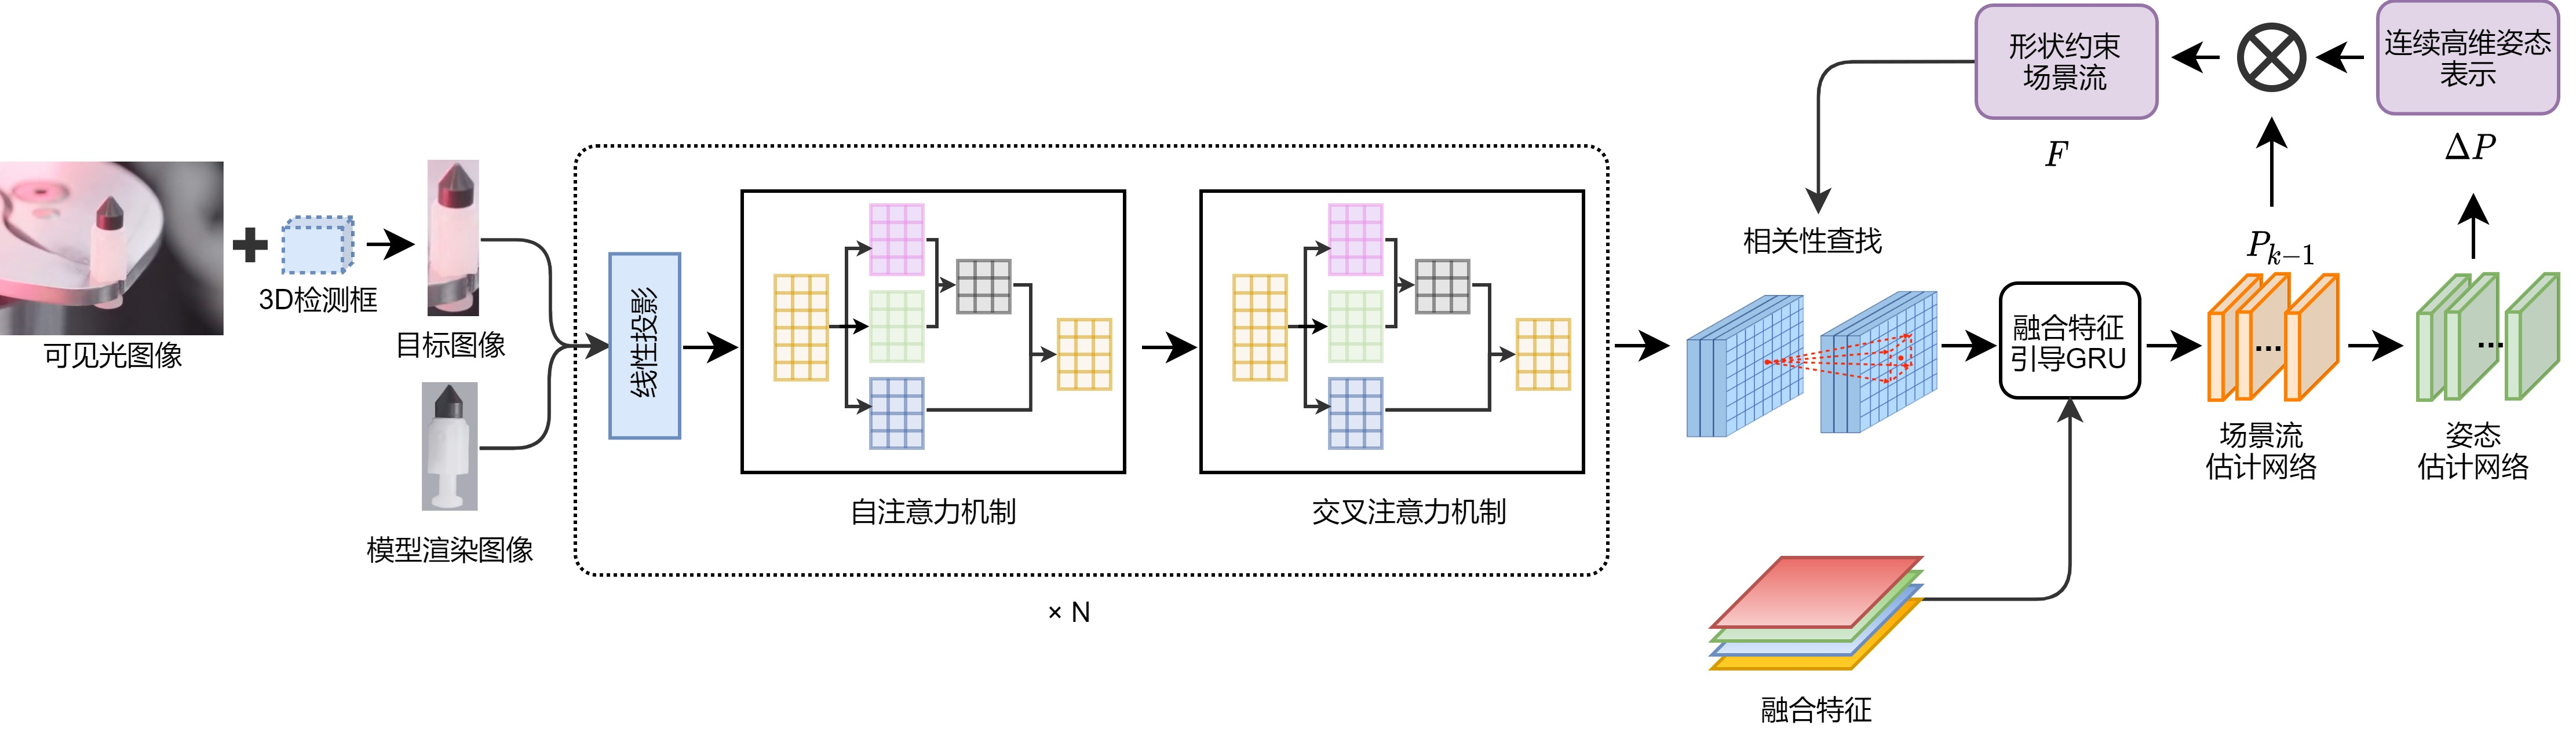
\includegraphics[width=0.9\linewidth]{figures/geo_guided_6d_refine.jpg}
    \caption{基于几何特征引导的6D姿态修正框架}\label{fig:geo_guided_6D_refine}
\end{figure}

本方案的关键问题在于对针对目标物体估计得到的不精确的6D姿态进行修正。目前基于2D匹配的6D姿态估计修正方案主要依赖于物体的纹理特征进行,没有考虑到物体的几何特征,因而不适用于弱纹理的目标。同时,当前方法在整个二维图像空间中搜索像素的匹配点,然而对于6D姿态估计来说,匹配点应该同样严格反映物体的形状,也就是满足3D几何约束。在无3D几何约束下进行搜索,搜索空间异常大,然而通过使用3D几何约束,我们可以将搜索空间限制在当前3D形状的所有二维投影点,进而缩小搜索空间。因此本方案提出基于几何特征引导的物体6D姿态修正框架,结合多源融合特征,通过物体的3D几何约束,引入物体的几何特征。



目前的6D姿态修正方法只利用一个光流估计网络来根据GRU更新后的当前状态信息来估计修正之后的2D密集匹配。然而,如前所述,这一范式只考虑到了物体的纹理特征,不适用于本方案的研究目标。
本方案提出通过使用额外的姿态估计网络,该网络的输入为修正之后的2D密集匹配与GRU的内部状态信息,并通过整合全局的局部对应关系来预测一个反映当前运动信息的相对姿态。
基于此,我们在每次迭代中预测一个相对姿态,通过累加得到最终的修正结果,我们的网络是端到端的,通过基于物体形状的损失函数来直接优化6D姿态,网络可以隐式的感知到物体的3D几何形状。


本方案的核心贡献是通过姿态引导光流来进行相关性查找。如图~\ref{fig:geo_guided_6D_refine}所示,光流估计网络得到的光流无法反映物体的形状,有很严重的畸变。因此我们提出通过能够严格反映物体形状的光流来进行相关性查找,进而在训练过程中,使网络感知到物体的3D几何形状。给定渲染图像的姿态以及当前估计的6D姿态,我们可以通过几何计算得到初始渲染图像中的每个像素在当前估计6D姿态下的对应点,也就是图~\ref{fig:geo_guided_6D_refine}中的姿态引导光流,能够严格反映物体的形状。同时,这种全局感知的方式能够修正一些不可靠的光流估计,进而得到与全局姿态相符合的对应点,进而使得这些像素迅速逃离局部解,缩小匹配时的搜索空间。

\textbf{整体框架}

本方案已经在基于光流的框架验证了方案的可行性。
首先利用目前成熟的 6D 姿态估计网络预测得到一个不精确的初始6D 姿态$P_0$,接下来利用该姿态对目标进行渲染和定位。
输入一张目标RGB图像与在初始姿态$P_0$下渲染的目标模型图像,本方案首先利用一个孪生卷积神经网络来对该两张图像进行特征提取,分别得到维度为$H\times W$的特征图$g_1$和$g_2$。
之后根据提取的特征向量构建4D相关体$C$,$C$的维度为$H\times W \times H \times W$,其中
\begin{equation}
    C_{ijkl} = g^1_{ij} \cdot g^2_{kl}
\end{equation}
$C$表示了$g_1$中所有特征向量与$g_2$中所有特征向量的相关性。
接下来,本方案在每次迭代中同时估计残差光流$\Delta F$与残差姿态$\Delta P$,并进行估计姿态的更新,即
\begin{equation}
    P_i = \Delta P_i \otimes P_{i-1}
\end{equation}
其中,本方案利用一个单独的姿态估计网络$f_{\theta}$来通过估计的残差光流进行残差姿态的回归,即
\begin{equation}
    \Delta P_i = f_{\theta}(\Delta F)
\end{equation}
$f_\theta$由若干个卷积层与全连接层组成,最终由两个支路分别预测旋转$\Delta R$与平移$\Delta t$。


残差光流估计的核心操作是通过相关性查找在4D相关体中在当前估计的2D密集匹配以及其周围邻域中进行索引,进而确定在当前估计的2D密集匹配下的相关性。
建立在深度特征的连续性假设上,朝着相关性更高的方向移动估计的对应点更可能找到目标对应点,因此通过在当前估计的光流基础上,估计一个偏移,使得估计对应点朝着相关性更高的方向移动。
本方案进一步借助于GRU,将相关性查找得到的相关性特征输入GRU中,以更新GRU内部的隐状态,进而利用GRU更新后的隐状态来进行残差光流的预测。
GRU被证明在序列任务建模中发挥着良好的作用,通过引入门控机制,选择性地保留或者舍弃先前的状态信息。

在初始方案的基础上,本方案扩展为基于RGB-D的数据输入场景下,提出基于场景流的6D姿态修正框架光流与场景流的区别在于,光流估计平面的二维运动,即估计源图像中每个像素在目标图像中的2D对应点。而场景流估计物体的三维运动,即估计源RGB-D图像中每个像素在目标图像中的3D对应点。
由于我们使用渲染技术合成初始姿态下的目标物体,相应的深度图$D$是可以得到的,因此可以通过几何推理的方式得到源图像中姿态$P_0$的物体到预测姿态$\hat{P}$下物体的场景流。

对于渲染图像中的一个像素$(u_1,v_1)$以及其相应的深度$d_1$,在已知渲染姿态以及相机内参的情况下,利用针孔相机模型反投影函数$\pi^{-1}$将其反投影到物体的CAD模型中,得到其对应的3D点$p=(x,y,z)$,
并将点$p$在预测姿态下$\hat{P}$进行投影即可得到其在$\hat{P}$下的对应点$(u_2,v_2)$以及其相应的深度$d_2$。
上述过程可以被表述为
\begin{equation}
    (u_2,v_2,d_2) = \pi(\pi^{-1}(u_1, v_1,d_1, k,P_0), k, \hat{p})
\end{equation}
其中$\pi$为针孔相机投影模型,即

\begin{equation}
    \begin{aligned}
    d
    \begin{bmatrix}
    u \\
    v \\
    1 \\
    \end{bmatrix}
    =K(Rp+t),
    \end{aligned}
\end{equation}
因此,场景流可以被表示为$\Delta u = u_2 - u_1, \Delta v = v_2 - v_1, \Delta d = d_2 - d_1$。
该场景流同样能够严格地反映物体的形状,进而将三维几何约束引入匹配过程,减小匹配时的搜索空间。
初始方案简单地使用光流进行相对姿态的回归,抛弃掉深度变化这一分量,仅从二维层面进行三维特征的回归,尽管可以通过数据驱动的学习方式将二维光流映射到三维空间,然而这是病态的,不利于网络的学习。
基于此,本方案进一步提出基于场景流的几何特征引导框架。在每次迭代中,网络回归残差场景流与残差姿态,将三维场景流进行投影到二维平面,得到形状约束的光流,利用目前成熟的二维相关性查找操作,来为残差场景流的估计服务。






\textbf{提取-匹配范式}

在光流估计场景下,更多地依赖于图像的浅层特征进行匹配。
然而,在本方案使用的场景下,不同的物体的往往呈现出不同的纹理与几何特征,网络需要更强的特征提取能力来提取到物体无关的特征,来为后续的匹配过程服务。
另外,初始方案中使用的编码器较为简单,提取出的特征不具有较强的表达性,这导致匹配过程的效率较低,往往依赖于多次迭代来进行优化,导致网络的运行速度较慢。
在本方案中,我们提出一种利用视觉注意力机制强大的特征提取能力和灵活的特征建模能力来提取得到足够具有表达性的特征。


注意力机制是一种基于查询$Q$、键$K$和值$V$向量的机制,通过计算查询向量和键向量之间的点积,得到每个值向量的注意力权重分布,从而实现信息传递。
具体地,注意力机制表示为:
\begin{equation}
    Attention(Q, K, V) = softmax(QK^T)V
\end{equation}
其中,softmax表示归一化函数,输出向量是值向量的加权和,其权重由相似度得分确定,从而实现了信息的选择性提取。
对于自注意力机制,对于输入的特征分别进行线性投影,得到$Q$,$K$和$V$。
对于交叉注意力机制,输入为两幅图像的特征$X_1$和$X_2$,对于$X_1$进行投影得到$Q$,对于$X_2$进行投影得到$K$和$V$。

本方案通过结合自注意力机制和交叉注意力机制,自注意力机制在每张图像内部通过特征交互进行特征增强,而交叉注意力机制在两张图像间进行特征交互,以获取两张图像的相关信息。
具体地说,自注意力机制通过计算每个位置的特征与其他位置特征的相似度来调整该位置的特征表示,以此实现特征增强。而交叉注意力机制则利用两张图像的相似性来加强它们之间的特征表示,从而实现后续更好的匹配。
这种基于注意力机制的特征增强方式不仅可以提高特征的表达能力,还可以在匹配过程中降低噪声干扰和错误匹配的概率,进一步提高了匹配的精度和鲁棒性。





\textbf{融合特征引导GRU}

本方案引入多源融合特征,利用融合特征进行GRU状态的更新。GRU的输入为相关性特征与融合特征,本方案将相关性特征与融合特征进行拼接,并将拼接后的特征输入到GRU进行状态的更新。相较于传统的单一特征,融合特征能够提供更丰富全面的信息,从而更好地描述
当前的物体,改善GRU的隐状态表示,为后续的场景流回归与姿态回归模型提供支持,进而提升姿态估计精度与效率。GRU的迭代方式可以表示为
\begin{equation}
    \begin{aligned}
        z_t &= \sigma(\mathrm{Conv}_{3\times3}([h_{t-1}, x_t], W_z)) \\
        r_t &= \sigma(\mathrm{Conv}_{3\times3}([h_{t-1}, x_t], W_r)) \\
        \hat{h}_t &= \mathrm{tanh}(\mathrm{Conv}_{3\times3}([r_t \otimes h_{t-1}, x_t], W_h)) \\
        h_t &= (1 - z_t)\otimes h_{t-1} + z_t \otimes \hat{h}_t
    \end{aligned}
\end{equation}
其中$h_t$即为更新后的隐状态,用来进行后续的场景流回归,$x_t$为相关性特征与融合特征的拼接。
GRU使用三个子网络分别建模遗忘信息的程度$z_t$、更新信息的程度$r_t$以及当前时刻的状态信息$\hat{h}_t$。
通过这三个子网络的交互,GRU可以有效地对迭代更新任务进行建模。

\textbf{姿态与场景流联合估计}

我们的方案使用经典的四元数作为旋转表示,并采用DeepIM中提出的分离相对姿态表示。
在联合优化光流和姿态时,优化姿态时的梯度反向传播对光流的优化也有益处。进一步修正光流可以提高姿态估计的精度,因此,良好的姿态表示在我们的框架中至关重要。
相对于绝对姿态,相对姿态的表示对网络的学习具有更高的要求,不合理的姿态表示会在网络的优化过程中引入不必要的困难。其中最重要的问题是坐标系的选取。DeepIM提出使用相机下物体的中心作为坐标系的中心,并使用与相机系的坐标轴平行的轴作为坐标系的中心。在这种表示下,旋转和平移得以解耦,适合网络的优化。

\begin{equation}
    \begin{aligned}
    \Delta x & = f_x(t_x^{i+1}/t_z^{i+1} - t_x^i/t_z^i)\\
    \Delta y & = f_y(t_y^{i+1}/t_z^{i+1} - t_y^i/t_z^i) \\
    \Delta z & = log(t_z^i/t_z^{i+1})
\end{aligned}
\end{equation}
其中,$f_x$与$f_y$为相机的焦距。在这种表示下,$v_x$与$v_y$被定义在图像平面上的位移,而$v_z$被定义为相对尺度的变化,网络可以从两张图像中物体的相对位置与大小推理得到。

然而,四元数旋转表示在欧几里得空间中是不连续的,不利于神经网络的回归。本方案提出将相对三维旋转映射到高维空间,以得到一个连续的相对旋转表示。
连续的目标函数可以提供更加稳定的梯度,进而加快相对姿态优化的收敛。
    




\NsfcSection{4}{本项目的特色与创新之处;}{}

本项目的特色和创新之处主要有三部分:
\myPara{多源融合表征的特色与创新之处}
危化品智能装配过程中不同零部件具有不同的光谱特征响应,通过引入光谱图像与可见光图像交叉注意力融合,弥补了可见光图像在危化品零部件细节特征提取上的不足。同时通过深度图像生成的点云特征与可见光图像特征的交叉融合得到补全点云全局特征,弥补了可见光图像三维几何信息的缺失。

\myPara{3D目标检测的特色与创新之处}
引入刚性感知检测方法,提出了一种新颖的基于距离函数的距离变换图来取代2D检测的图像掩膜标注以及3D点云的逐点分割掩膜,并利用距离变换图指导网络在训练期间仅由目标可见部分的正特征单元监督而不受遮挡部分的干扰;引入2D候选引导的3D候选融合策略来对3D检测候选置信度进行处理,并且设计了融合候选局部预测的方法避免非最大抑制方法对正确检测候选的抑制,以产生更准确的检测结果。
\myPara{基于目标几何特征引导的6D位姿估计的特色与创新之处}
通过可微相对姿态求解层逐步优化估计的6D姿态,并将几何信息引入特征匹配过程,使得匹配得到的特征与物体的几何形状一致。进一步显式地使用深度神经网络编码几何特征作为姿态修正网络的参考信息。

\NsfcSection{5}{年度研究计划及预期研究结果}{(包括拟组织的重要学术交流活动、国际合作与交流计划等)。}

\subsection{年度研究计划}

本课题研究期限从2024年1月到2027年12月。年度计划如下:  

2024.01-2024.06,构建本项目专用数据集。选定特定危化品类型,通过实验获得最佳光谱谱段。将智能装配车间的可见光相机位置,增加深度相机和光谱相机。捕获装配目标场景下的深度图像和光谱图像。完成可见光影像、深度图和光谱影像之间的配准,并清洗数据,构建完整可用的多模态融合数据集。拟发表国际期刊论文1\textasciitilde2篇,形成的数据集对学术界开放下载和使用。

2024.07-2025.02,可见光图与深度图的主从式深度网络结构。在目标检测阶段,选择合适的Backbone作为主干,提取可光图像的特征,同时降低深度特征提取网络的深度,研究合适的特征交叉和融合方式。拟发表国际期刊论文2\textasciitilde3篇,其中包括一篇国际顶会论文,参加国际会议与同行交流。

2025.03-2025.12,光谱图像特征的集成融合网络结构研究。分析光谱特征提取的transformer结构输出特征与可见光、深度图特征的有效融合方法。拟发表国际期刊论文2\textasciitilde3篇,其中包括一篇国际顶会论文,参加国际会议与同行交流。

2026.01-2026.06,有遮挡情况下的3D目标鲁棒检测算法研究。拟发表国际期刊论文2\textasciitilde3篇,其中包括一篇国际顶会论文,参加国际会议与同行交流。

2026.07-2027.03,基于工件几何特征引导的位姿修正方法研究。拟发表国际期刊论文2\textasciitilde3篇,其中包括一篇国际顶会论文,参加国际会议与同行交流。

2027.04-2027.12,工件无纹理和有遮挡情况下的算法适应性实验,分析精度误差来源,进一步改进位姿修正方法,提升算法在真实场景下的精度和鲁棒性。拟发表国际期刊论文2\textasciitilde3篇,其中包括一篇国际顶会论文,参加国际会议与同行交流。

\subsection{预期研究成果}

预期发表学术研究论文15篇,其中顶会或顶刊论文10篇,申请专利和软件著作权10件,公开研究数据集一套,培养博士研究生1\textasciitilde2名,硕士研究生3\textasciitilde5名。


%%%%%%%%%%%%%%%%%%%%%%%%%%%%%%%%%%%%%%%%%%%%%%%%%
\ContentDes{(二)研究基础与工作条件}

\NsfcSection{1}{研究基础}{
(与本项目相关的研究工作积累和已取得的研究工作成绩);}

\subsection{工作基础}


\myPara{位姿估计方面}申请人团队2023年录用了两篇IEEE国际顶会CVPR论文,其中一篇为“Yang Hai, Rui Song, Jiaojiao Li, Mathieu Salzmann, Yinlin Hu. Rigidity-Aware Detection for 6D Object Pose Estimation. IEEE CVPR2023 \#2298”,另一篇为“Yang Hai, Rui Song, Jiaojiao Li, Yinlin Hu. Shape-Constraint Recurrent Flow for 6D Object Pose Estimation. IEEE CVPR2023 \#2307”。

\myPara{深度图的点云处理方面}申请人团队在点云分类、语义分割、点云补全等点云处理主流任务上开展研究,在相关领域国际顶会与核心期刊上发表高水平论文四篇,其中申请人团队2022年在相关领域国际高水平期刊上发表SCI论文三篇,其中一篇为“Fengda Hao, Jiaojiao Li*, Rui Song*, Yunsong Li and Kailang Cao. Structure-Aware Graph Convolution Network for Point Cloud Parsing.”发表在计算机视觉领域中科院一区期刊《IEEE Transactions on Multimedia》上;一篇为“Fengda Hao, Rui Song*, JiaoJiao Li*, Kailang Cao, Yunsong Li. Cascaded Geometric Feature Modulation Network for Point Cloud Processing.”发表在计算机学科国际学术期刊《Neurocomputing》上,一篇为“Fengda Hao, Jiaojiao Li, Rui Song, Yunsong Li and Kailang Cao. Mixed Feature Prediction on Boundary Learning for Point Cloud Semantic Segmentation.”发表在遥感领域权威期刊《Remote Sensing》上。另外,申请人团队在国际计算机多媒体领域顶级会议ACM Multimedia 2021上发表题为“ASFM-Net: Asymmetrical Siamese Feature Matching Network for Point Completion”的研究成果。该项成果在2021年斯坦福大学发布的Completion3D点云补全任务榜单中排列第一。

\myPara{光谱图像目标检测方面}
目标检测:申请人团队在遥感图像目标检测领域开展研究,在相关领域国际期刊上发表了高水平论文,其中申请人团队2022年在相关领域国际高水平期刊上发表数篇SCI论文,代表性论文有“J. Li, H. Zhang, R. Song, W. Xie, Y. Li and Q. Du, Structure-Guided Feature Transform Hybrid Residual Network for Remote Sensing Object Detection.”发表在遥感领域中科院一区TOP期刊《IEEE Transactions on Geoscience and Remote Sensing》上,该工作提出了一种新的结构引导的特征变换混合残差(SGFTHR)网络,该网络可以以无锚的方式克服在不同尺度上目标检测的低性能,尤其是对于小而密集的目标,进一步提升了检测性能。

\myPara{多源融合方面}
多源融合:申请人团队在多源数据融合处理领域展开研究,在相关领域国际核心期刊上发表高水平论文三篇,其申请人团队2022年在相关领域国际高水平期刊上发表SCI论文三篇,其中一篇为“Jiaojiao Li,Yuzhe Liu, Rui Song, Yunsong Li, Kailiang Han and Qian Du. Sal2RN: A Spatial–Spectral Salient Reinforcement Network for Hyperspectral and LiDAR Data Fusion Classification”发表在遥感图像处理领域中科院一区TOP期刊《IEEE Transactions on Geoscience and Remote Sensing》上,本文提出了一种基于跨层特征提取和互补融合策略的深度学习网络用于LiDAR和Hyperspectral联合分类,提升了LiDAR和Hyperspectral的分类性能;一篇为“Jiaojiao Li, Yinle Ma, Rui Song, Bobo Xi, Danfeng Hong and Qian Du. A Triplet Semi-supervised Deep Network for Fusion Classification of Hyperspectral and LiDAR Data” 发表在遥感图像处理领域中科院一区TOP期刊《IEEE Transactions on Geoscience and Remote Sensing》上,提出一种级联神经网络来提取LiDAR深度特征,提升了LiDAR和Hyperspectral图像的融合感知性能;一篇为“Yunsong Li , Yuxuan Zheng, Jiaojiao Li, Rui Song. Hyperspectral Pansharpening With Adaptive Feature Modulation-Based Detail Injection Network”, 发表在遥感图像处理领域中科院一区TOP期刊《IEEE Transactions on Geoscience and Remote Sensing》上,提出一种基于自适应特征调制的细节注入融合网络,提升PAN和Hyperspectral的融合性能。


\subsection{研究工作获奖}

\myPara{ECCV2022 BOP 6D姿态估计挑战赛单模型赛道冠军}
申请人团队在计算机视觉顶级会议ECCV 2022举办的BOP 6D位姿估计挑战赛中获得了最佳单模型奖项“The Best Single-Model Method”(链接地址\url{https://cmp.felk.cvut.cz/sixd/workshop_2022/slides/bop_challenge_2022_results.pdf}),竞赛中提出的方法可以同时处理单目RGB以及RGB-D图像,可扩展性较强。

\myPara{2019年中央军委“天智杯”人工智能挑战赛冠军}
申请人团队2019年12月19日参加了由军委装备发展部指导,航天系统部主办的我国首届“天智杯”人工智能挑战赛。挑战赛题目是以主办方提供的光学卫星遥感影像为处理对象,难点为全色影像与RGB影像同时存在,且在大场景范围影像中同时完成四类典型地物要素的像素级分割,获得地物要素精确轮廓边缘和属性信息,申请人团队针对数据特点,创新性提出了空间-通道最大化注意力机制为核心的网络模型,并使用了决策级融合和特征级融合的策略,最终得到了精确且鲁棒性的分割结果,在科目二竞赛中获得第一名。

\NsfcSection{2}{工作条件}{
(包括已具备的实验条件,尚缺少的实验条件和拟解决的途径,包括利用国家实验室、国家重点实验室和部门重点实验室等研究基地的计划与落实情况);}


\myPara{经费和硬件条件方面}我们


\myPara{人员方面}我们

\myPara{国内外合作方面} 我们


\NsfcSection{3}{正在承担的与本项目相关的科研项目情况}{
(申请人和主要参与者正在承担的与本项目相关的科研项目情况,包括国家自然科学基金的项目和国家其他科技计划项目,要注明项目的资助机构、项目类别、批准号、项目名称、获资助金额、起止年月、与本项目的关系及负责的内容等);}

已获批一项陕西省重点研发计划“科学家+工程师”队伍建设项目,项目名称为《航天装备智能制造“科学家+工程师”队伍》,公示链接\url{https://kjt.shaanxi.gov.cn/kjzx/tzgg/296970.html},项目资助总金额为30万元,起止年月为2023年1月至2025年12月。该项目为申请人团队与西安航天自动化股份有限公司联合申报的团队建设项目,主要经费用于企业硬件平台的搭建。西安航天自动化股份有限公司是我国航天特种装备的主要生产企业,在该项目的支持下,申请人团队将在企业产线上搭建一套完整的多模态融合采集硬件平台,为本项目的顺利执行打好基础。本项目研发的成果,也将应用于合作企业的实际智能装备生产流程中,为我国的智能制造装备升级提供理论支撑。


\NsfcSection{4}{完成国家自然科学基金项目情况}{
(对申请人负责的前一个已资助期满的科学基金项目(项目名称及批准号)完成情况、后续研究进展及与本申请项目的关系加以详细说明。另附该项目的研究工作总结摘要(限500字)和相关成果详细目录)。}

补充中...

%%%%%%%%%%%%%%%%%%%%%%%%%%%%%%%%%%%%%%%%%%%%%%%%%
\ContentDes{(三) 其他需要说明的问题}



\NsfcSection{1}{}{
申请人同年申请不同类型的国家自然科学基金项目情况(列明同年申请的其他项目的项目类型、项目名称信息,并说明与本项目之间的区别与联系)。}

同年参与另外一项自然科学基金面上项目的申请,项目类型为面上项目,项目名称为...

该项目与本项目的侧重点不同。

\NsfcSection{2}{}{
具有高级专业技术职务(职称)的申请人或者主要参与者是否存在同年申请或者参与申请国家自然科学基金项目的单位不一致的情况;如存在上述情况,列明所涉及人员的姓名,申请或参与申请的其他项目的项目类型、项目名称、单位名称、上述人员在该项目中是申请人还是参与者,并说明单位不一致原因。}

无。

\NsfcSection{3}{}{
具有高级专业技术职务(职称)的申请人或者主要参与者是否存在与正在承担的国家自然科学基金项目的单位不一致的情况;如存在上述情况,列明所涉及人员的姓名,正在承担项目的批准号、项目类型、项目名称、单位名称、起止年月,并说明单位不一致原因。}

无。

\NsfcSection{4}{}{其他。}

无。


\end{document}
